\documentclass[a4paper,11pt]{book}
\usepackage[T1]{fontenc}
\usepackage[utf8]{inputenc}
\usepackage{lmodern}
\usepackage{hyperref}
\usepackage{graphicx}
\usepackage[english]{babel}
\usepackage{fancyvrb}
\usepackage{mathtools}
\usepackage{qtree}
\usepackage{pgfplots}

%%%%%%%%%%%%%%%%%%%%%%%%%%%%%%%%%%%%%%%%%%%%%%%%%%%%%%%%%%%%%%%%%%%%%
% 'dedication' environment: To add a dedication paragraph 
% at the start% of book
% Source: http://www.tug.org/pipermail/texhax/2010-June/015184.html
%%%%%%%%%%%%%%%%%%%%%%%%%%%%%%%%%%%%%%%%%%%%%%%%%%%%%%%%%%%%%%%%%%%%%
\newenvironment{dedication}
{
   \cleardoublepage
   \thispagestyle{empty}
   \vspace*{\stretch{1}}
   \hfill\begin{minipage}[t]{0.66\textwidth}
   \raggedright
}
{
   \end{minipage}
   \vspace*{\stretch{3}}
   \clearpage
}

%%%%%%%%%%%%%%%%%%%%%%%%%%%%%%%%%%%%%%%%%%%%%%%%
% Chapter quote at the start of chapter        %
% Source: http://tex.stackexchange.com/a/53380 %
%%%%%%%%%%%%%%%%%%%%%%%%%%%%%%%%%%%%%%%%%%%%%%%%
\makeatletter
\renewcommand{\@chapapp}{}% Not necessary...
\newenvironment{chapquote}[2][2em]
  {\setlength{\@tempdima}{#1}%
   \def\chapquote@author{#2}%
   \parshape 1 \@tempdima \dimexpr\textwidth-2\@tempdima\relax%
   \itshape}
  {\par\normalfont\hfill--\ \chapquote@author\hspace*{\@tempdima}\par\bigskip}
\makeatother

%%%%%%%%%%%%%%%%%%%%%%%%%%%%%%%%%%%%%%%%%%%%%%%%%%%
% First page of book which contains 'stuff' like: %
%  - Book title, subtitle                         %
%  - Book author name                             %
%%%%%%%%%%%%%%%%%%%%%%%%%%%%%%%%%%%%%%%%%%%%%%%%%%%

% Book's title and subtitle
\title{\Huge \textbf{A Pamphlet against R} \\ \huge{Computational Intelligence in Guile Scheme}}
% Author
\author{\textsc{Panicz Maciej Godek}}

\begin{document}

\frontmatter
\maketitle


%%%%%%%%%%%%%%%%%%%%%%%%%%%%%%%%%%%%%%%%%%%%%%%%%%%%%%%%%%%%%%%%%%%%%%
% Auto-generated table of contents, list of figures and list of tables
%%%%%%%%%%%%%%%%%%%%%%%%%%%%%%%%%%%%%%%%%%%%%%%%%%%%%%%%%%%%%%%%%%%%%%
\tableofcontents

\mainmatter

%%%%%%%%%%%
% Preface %
%%%%%%%%%%%
\chapter*{Preface}

\begin{chapquote}{Anyone who hates all the stupid quotes
at the beginning of each chapter}
``I hate all those stupid quotes at the beginning of each chapter.''
\end{chapquote}


Behind every text, however technical, there is a personal story of
its author\footnote{Even if the text was generated by a machine, and
the machine was designed by a computer program, and so on, this causal
chain eventually has its author.} and the author's motivations.

Having worked for a couple of months in an engineering company that
manufactured electronic equipment, I decided that perhaps its the
best time to finish my education. I enrolled to the department of
Computer Science at the University of Gdańsk. Among other subjects,
we had a lab devoted to some data processing heuristics jointly named 
``computational intelligence''.

During the first meeting, we were getting acquainted with the
programming language R that we were supposed to use throughout
the semester for the assignments.

Initially, I had an ambivalent attitude towards this endeavour.
On one hand, there's been quite a few programming languages
that I used throughout my career: JavaScript, Python, PHP,
Perl, Bash, Matlab, SQL, C, C++, Assembly, Haskell, Erlang, Prolog,
Pascal, BASIC, VisualBasic, MiniKanren and a few others. Some of those
languages were really mind-expanding in some ways.

On the other hand, being a rather seasoned Schemer, I knew that
most of these languages were only inferior incarnations of Lisp,
and I could find little value in learning a new syntactical disguise
for the well-established concepts.

I was very soon to find out that my skepticism was right, and that
learning R would require interiorizing a lot of unfortunate
idiosyncrasies that the authors of the language picked for their
own reasons, and that I would constantly stumble over
incomprehensible limitations and discrepancies between common
practices and the language developers' decisions. And for that
I didn't want to waste my time.

Bjarne Stroustrup said that there are only two kinds of languages:
the ones people complain about and the ones nobody uses\footnote{He
probably said that, because he was himself a creator of a popular
language that everybody complains about.}. The advocates of R sometimes
admit that perhaps the language itself isn't perfect, but it contains
a lot of convenient libraries that make the whole system worthwhile.

Being a nobody, I was in a comfortable situation, because I could
decide whether I want to complain on a language or not. I asked
my TA whether he would allow me to choose another language for doing
the assignments, and he agreed.

My language of choice was of course Scheme, or -- more precisely --
Guile Scheme. I chose Guile Scheme because it has a wonderful trait:
rather than complaining on the features that I don't like, I can
replace them in the way that I find more suitable. If a feature is
lacking from the language, I can add it, rather than swear and curse
its developers.

The title of this pamphlet may suggest that it is written against
the R programming language, but it is actually written against the
majority of programming languages in use today\footnote{
However, the case of the R programming language is particularly
interesting, because initially it was just a harmless implementation
of Scheme, but then as a result of irresponsible experiments
of mad scientists it got mutated into a monster\cite{Ihaka2010}.}.
The ultimate goal of this text is to kill them.

Having recognized that the aforementioned is rather unlikely
to achieve, I will be satisfied if it anyone finds any value in
this pamphlet, whether it be education, entertainment or personal
hygiene\footnote{Concerns the printed copies}.

\section*{Structure of this pamphlet}
This pamphlet assumes no prior knowledge about programming.
If you think that you already possess that sort of knowledge,
that's not my problem. 

Throughout the subsequent chapters, a large subset of the Scheme
programming language is being laid out, and the later chapters
usually dwell upon the knowledge from the previous ones.
The first chapter introduces all the elementary notions needed
for programming. The next two chapters show how to use that
knowledge in practice. The fourth chapter introduces a few
more features of the language that are used in the fifth
chapter.

In each chapter there also appear some new definitions that
are used later. For example, the third chapter presents
the notion of \texttt{equivalence-classes}, that are used
extensively throughout the fifth chapter.

The vision of programming presented here departs significantly
from the mainstream view, where a program is perceived
as a sequence of steps that lead us to a desired goal.

On the contrary, I intended to explain programs as
intellectual constructs of increasing complexity,
so reading the chapters in their proper sequence
is strongly recommended.

\section*{How to read this pamphlet}

The essential part of the pamphlet are the definitions.
Everything else is just a scaffolding whose purpose is to
facilitate their comprehension. The ultimate goal is to
make those definitions dance in the reader's head, so
each definition should be studied with care. If there are
no examples given, it is up to the reader to come up
with proper examples, because if a definition is the
dance, then examples are certainly the ones that
perform that dance.

The whole point of a definition is to create or express
a notion that can be further used to think about phenomena
in the world. Internalizing a definition is not always
a pleasant task, because it requires an intellectual
effort of focusing and remembering.

Reading programs isn't like reading novels, because
of their higher level of generality: we can absorb
stories almost effortlessly, but comprehending abstractions
requires a very different attitude. Well written programs
are a bit like mathematical textbooks. The latter usually
consist mainly of definitions, examples, theorems and proofs
(and excercises).

The role of theorems is usually diminished in the realm
of computer programs: the essential part are the constructions,
the definitions. Examples (sometimes called \textit{unit
tests} by the software folks) serve mainly as a means
of ensuring that a program behaves as expected, which
gains importance as the program is subject to a change.
Theorems manifest themselves in a weak form of \textit{assertions}
and \textit{type signatures}, and proofs are usually performed
by specific tools such as type checkers or model checkers.
Furthermore, false assertions can typically be refuted
during the execution of a program.

In the case of the math textbooks, exercises and examples
are a way of facilitating comprehension. It is usually
much easier to understand an abstract definition if
we have can train it on a given example, while exercises
are ``partial examples'' that enforce us to do the
reasoning for ourselves.

Reading a math textbook without exercises is also
possible, but it is up to the reader to come up
with those\footnote{
Programmers usually read computer programs in order
to change them, which is an ultimate exercise
in the comprehension of complex systems. On the
other hand, programs are often written with the
purpose of ``doing their job'', rather than
being comprehended and modfied.

From my experience, this approach dominates
not only in the industry (which is understandable),
but also in education (which is harmful to the
industry).
}.

\section*{Who should read this pamphlet}

The title of this pamphlet may be misleading,
because it may cause readers to think that
it mainly concerns some computational methods.
Although there are certainly some computations
involved, the pamphlet is really about thinking
and communicating thoughts.

While it is difficult to imagine a person that
wouldn't potentially benefit from obtaining the
knowledge presented here, there are some groups
of people that are particularly encoraged to do so.

For instance, this text may be of interest to
philosophers and linguists, because it presents
a linguistic perspective on communicating thoughts
in a precise manner.

It may also be interesting to evolutionary biologists,
because it contains a quote from Richard Dawkins
and stuff like that.

It should be of particular interest to computer
scientists and programming language designers, to
convince them to stop designing new languages immediately,
because -- as the history teaches us -- they sometimes
succeed, forcing generations of programmers to
suffer because of the ignorance of their creators.

However, as I said, this book is no more about
programming than it is about clear thinking, and
it is difficult to imagine someone that could not
benefit from this ability.

So perhaps the shortest answer to the question posited
in the title of this section is: \textit{you}.

\section*{Acknowledgements}
Most of all, I would like to thank Grzegorz Madejski, who was
the teaching assistant that allowed me to go my own way,
and encouraged me to devote more time to this project.

I am also truly grateful to my family and my girlfriend,
as they all encouraged me to go back to the university. I certainly
wouldn't make it without their support.

I deeply appreciate the interest, support, feedback and
encoragement of my friends who allowed me to bother them with
the early versions of this text, and with whom I have had many
valuable and inspiring conversations, including Ścisław Dercz,
Hubert Melchert, Michał Janke, Marcin Jędruch, Jan Makulec
and Aleksander Mohuczy-Dominiak. 

Last and the least, I would like to thank Bjarne Stroustrup,
Rasmus Lerdorf and all the others who fueled me with hatred
needed to finish this lousy piece of work.

\section*{Reporting bugs}

I realize that the quality of this text may be questionable.
After all, this is a pamphlet. However, if you find any parts
of the text obscure or difficult to understand, or if you
find any mistakes in the explanations presented here, or
simply want to talk about how miserable the world is, feel
free to write an e-mail to \url{godek.maciek+pamphlet@gmail.com}.

Also make sure that you are reading the latest version
of this pamphlet, always available from

\url{https://panicz.github.io/pamphlet/pamphlet.pdf}

as many of the bugs may already have been fixed.

%%%%%%%%%%%%%%%%
% NEW CHAPTER! %
%%%%%%%%%%%%%%%%
\chapter{Introduction}

\begin{chapquote}{Hal Abelson and Gerald Sussman, 
\textit{Structure and Interpretation of Computer programs}}

  ``The acts of the mind [...] are chiefly these three:
  1. Combining several simple ideas into one, and thus all complex
  ideas are made.
  2. [...] bringing two ideas, whether simple or complex, together,
  and setting them by one so as to take a view of them at once,
  without uniting them into one, by which it gets all its ideas
  of relations.
  3. [...] separating them from all the other ideas that accompany
  them in their real existence: this is called abstraction, and thus
  all its general ideas are made.''

  John Locke, \textit{An Essay Concerning Human Understanding} (1690)

  [...]

  A powerful programming language [...] serves as a framework within 
  which we organize our ideas [...]. Every programming language has
  three mechanisms for accomplishing this:
  - \textbf{primitive expressions} [...]
  - \textbf{means of combination} [...]
  - \textbf{means of abstraction} [...]

\end{chapquote}

\section{Epistemic role of programming}

This text was written with the belief that programming
is not only a way of automating common repetitive tasks,
but -- most importantly -- it is a means (probably the most
efficient) of representing knowledge and understanding
the world and its phenomena, as well as expressing original
ideas.

This view is frequently obscured by some bad practices
that are widespread among programmers. Apart from expressing
knowledge and ideas, programming languages allow programmers
to do virtually everything they like -- it is therefore
possible that they write code which gets in the way to
understanding, rather than facilitate it\footnote{Apparently
even excellent programmers and great erudites have been failing 
at this task. One of the most extreme examples is the code from 
Donald Knuth's \textit{The Art of Programming}.
Written in the \texttt{MIX} assembly, the code only hides the
conceptual structure of presented solutions from the reader.}.

The claim that many programmers write code in ``the wrong way'',
and that the author of this pamphlet knows which way is 
``the right way'' may seem pretentious. It must therefore
inevitably be left to the reader to judge whether the author's
claims are true.

\subsection{Expression-based programming}

Throughout this pamphlet, we will be perceiving computer programs
as constructions of compound objects. This view has recently been
gaining more popularity, but it is still far from the mainstream
view, which claims that a program is a set of instructions that
ought to be performed in a given order.

The latter view is often called \textit{imperative programming},
and has traditionally been contrasted with \textit{declarative
 programming}.
Within the realm of declarative programming, there is a particular
subset called \textit{functional programming}, where the programmer
creates programs by defining functions (in mathematical sense).

However, since the notion of functional programming has recently
been somewhat appropriated by Haskell, and for some reasons that
shall become clear later, I will prefer to use the term
\textit{expression-based programming} or \textit{constructive
programming}.

For example, let's say that someone wishes to write a program that
computes \textbf{a sum of squares of initial seven prime numbers}. 
The imperative program that does this could look as follows:

%\lstset{language=Python}
\begin{Verbatim}[samepage=true]

counter := 7
number := 0
sum := 0
while(counter > 0):
    if is_prime(number):
        sum := sum + number^2
        counter := counter - 1
    number := number + 1

\end{Verbatim}
%\lstset{language=Lisp}

After its execution, the \texttt{sum} variable will contain the
desired value.

However, if we take a look at the specification of the problem,
we will notice that it can be itself perceived as a part of the
solution: the expression ``sum of squares of initial seven prime
 numbers'' has a certain linguistic (or syntactic) structure,
and a corresponding conceptual (or semantic) structure. The 
syntactic structure may not be immediately apparent, but simple
analysis shows that the outer form of the expression is 
``sum of $X$'', where $X$ is ``squares of initial seven prime
numbers''. We can further decompose the latter, extracting the 
form ``squares of $Y$'',  where $Y$ is ``initial seven prime 
numbers''. Making yet another step, we obtain the expression
``initial $N$ prime numbers'', where $N$ is ``seven''.

\begin{center}
\Tree [.sum 
  [.squares 
    [.prime-numbers initial seven ] ] ]
\end{center}

This isn't the only way in which we can perform decomposition.
That's because the natural language that we use in our everyday
communication is naturally ambiguous. For instance, by 
``initial seven prime numbers'', do we mean ``a set of initial
 prime numbers'', or ``a sequence of initial prime numbers''?

This distinction is of course insignificant from the point of view of
our task, because addition is commutative, and hence the order in which
we compute this sum is arbitrary. On the other hand, if we asked
someone to name the initial seven prime numbers, it would be likely
that he or she would enumerate them in the ascending order. If we
investigated further into that phenomenon, it would probably turn
out that the order is a consequence of the order in which the numbers
are computed by the speaker. Indeed, what a shocking experience it
would be to hear those numbers being uttered in a random or descending
order!

In order to avoid such shocks, people apply the so-called
\textit{cooperative principles} to their conversations\footnote{
The theory of Cooperative Principles was formulated by Paul Grice.
He explicated four maxims that ought to be applied in effective
communication. Probably the most relevant to programming and
the one that is least respected by programmers is the Maxim
of Manner, which recommends to avoid obscurity of expression,
avoid ambiguity, be brief and be orderly.}: they
try to adopt their utterances to the expectations of their
interlocutors (to the extent in which they can recognize them),
or -- in the parlance of programmers -- they ``try to design
clean and simple APIs''\footnote{Seriously.}.

Note however, that even if there is no natural order of elements
in a set, whenever we wish to enumerate elements from that set,
imposing \textit{some} order is inevitable.

Therefore, unless specified otherwise, whenever we speak about
some multitude of elements, we shall mean a sequence of those
elements, rather than a set (even if the order is irrelevant).

Returning to our example, we have a function ``initial $N$
prime numbers'', where $N$ is a natural number. The value
of a function, for a given $N$, is an ascending sequence
of $N$ initial prime numbers. For instance, the value (or meaning
\footnote{As it was shown by Frege, the word ``meaning'' is also
ambiguous, and can either mean \textit{intension/connotation} or 
\textit{extension/denotation}.
Intension of a semantically compound concept is its formulation
in simpler terms.}, or denotation) of expression ``initial 7 
prime numbers'' is a sequence \texttt{(2 3 5 7 11 13 17)}
\footnote{Of course, we cannot write down a sequence, and so we are 
forced to write down a \textit{textual representation} of a sequence.
In fact, we can only write down two distinct textual expressions,
hoping that the reader will establish in her or his mind, that those
distinct two expressions are meant to refer to the same abstract
object.}.

This is as far as we can go with the linguistic analysis.
Obviously, the expressions under consideration consist of
words, but their meanings do not (at least not in this
particular case)\footnote{It is possible to build linguistic
expressions whose meanings consist of words. A fine example
is a linguistic expression ``This sentence'', which refers
to a sequence of two words: \texttt{(This sentence)}.}:
the sequence of numbers consists of numbers and their order.
We could therefore ask: what is the structure of a sequence?

We can note that sequences can be empty, as it is the case
with the denotation of the expression ``initial 0 prime numbers'',
or ``empty sequence''. Non-empty sequences can be decomposed
into their first element, and the remainder of its elements
(which may be empty). This prompts us with a recipe to construct
sequences recursively. First, let's note that the phrase
``initial $N$ prime numbers'' is synonymous with ``$N$ least
prime numbers greater than 0''. Therefore we have function
of two arguments: ``$N$ least prime numbers greater than $M$''.

We can define this function as follows:

The meaning of ``$0$ least prime numbers greater than $M$''
is an empty sequence.

The meaning of ``$N+1$ prime numbers greater than $M$''
is a sequence whose first element is $M+1$, and whose
remaining elements are the $N$ prime numbers greater
than $M+1$, if $M+1$ is a prime number. Otherwise
it's just the same as $N+1$ prime numbers greater than $M+1$.

Although the above formulation is a legitimate description
that explains how to construct a sequence of subsequent
prime numbers, it disconcertingly brings legal gibberish
to mind. It also makes it difficult to distinguish between
the strict definitional part of the text from its more
explanatory fragments. Moreover, as it was noted before,
the syntactical structure of the text isn't immediately
clear even for the simplest examples.

In order to handle these issues, it is customary to
introduce a formal notation. It is a common practice
in mathematics, where mathematicians use special symbols
to denote certain abstract concepts, and in logic, where
logicians try to make certain reasonings more explicit.

\section{Introduction to Scheme}

In the quest for our perfect notation, we shall stick
to the rule of parsimony: we want to make as few assumptions
and conventions as possible, but we also want to make sure
that they are universal. Firstly, let's embrace the
compound syntactical units in parentheses. Then, the
expression ``sum of squares of initial seven prime numbers''
becomes:

\texttt{(sum (squares (initial seven prime numbers)))}

While at first the parentheses may seem difficult
to match, they allow to avoid confusions and ambiguities
that are typical for the natural language. Note also,
that we got rid of the ``of'' prepositions, because
they provide no information: we can simply read \texttt{(f x)}
as ``$f$ of $x$'' (provided that $f$ has only one argument).

Furthermore, let's stick to a convention, that a single
concept is expressed using a single word, where by words
we mean sequences of letters separated with parentheses
or white spaces. Also, let's make sure that the ruling
word of the expressions appears at the first position.
We can make compound words using hyphens:

\texttt{(sum (squares (prime-numbers initial seven)))}

This formulation expresses the structure of our problem
well enough using so-called \textit{fully parenthesized
Polish notation} -- certainly we can no longer be confused
with lawyers. Now the only thing that's left is to explain
in basic terms what we mean by \texttt{sum}, \texttt{squares}
and \texttt{prime-numbers}. The question which terms
are to be regarded as basic depends on the context.
In this particular case, we also happen to have written
(a fragment of) a program in a programming language called Scheme,
which enumerates a whole set of notions that are regarded as 
simple\footnote{The exact specification of the basic terms
of Scheme is provided in the \textit{Revised$^n$ Report on the
Algorithmic Language Scheme} that can be found at
\url{http://www.schemers.org/Documents/Standards}.}, and the notion of
\texttt{prime-numbers} certainly does not belong to that set.
It does, however, contain the notions of numbers, addition,
multiplication, division, comparison and it also provides some means
to construct and deconstruct sequences. Most importantly,
it provides means for defining new notions.

\subsection{Constructions}

Travestying our construction of ``least $N$ prime numbers 
greater than $M$'' from previous section, we can write:

\begin{Verbatim}[samepage=true]
(define (prime-numbers amount from)
  (if (= amount 0)
    '()
    (if (prime? from)
      (cons from (prime-numbers (- amount 1) (+ from 1)))
      (prime-numbers amount (+ from 1)))))
\end{Verbatim}

Although conceptually we present nothing new here compared to
the previous section, there are a few formal elements that need
to be explained. First of all, we use a special \texttt{define}
form from the Scheme language. This way, we give a name
to the new concept that we are defining\footnote{Although the
concept might not be so new for us, because we have defined
it informally in the previous section, it certainly is new for
the Scheme interpreter.}. We also observe that there are
quite a few new concepts used in the definition. The body (or
\textit{definiens}, if you please) consists of an \texttt{if}
expression, which -- in general -- takes the following form:

\texttt{(if <condition> <then> <else>)}

The value of the \texttt{if} expression depends on the value
of \texttt{<condition>}. If it is true in a given context, then
the value of the whole expression becomes the value of the 
\texttt{<then>} expression. Otherwise, it is the value of the
\texttt{<else>} expression. (This is actually quite straightforward,
if you think about it.)

The expression that appears as the \texttt{<condition>} has 
a form \texttt{(= amount 0)}. The meaning of the word \texttt{=} is
the \textit{numerical comparison}, commonly found in mathematics. It
can be surprising to see it used as \texttt{(= x y)} rather
than \texttt{(x = y)}. Recall however our convention that
``the ruling word of the expression appears at the first
position''. We could depart from that rule for mathematical
expressions (and whoever knows where else), but this would
only make our rule set more complex. However, it actually
turns out that mathematical expressions do not appear so
frequently in computer programs to make it worth the trouble,
and having a simple language turns out much greater an
advantage.

As one can expect, the \texttt{(= amount 0)} expression evaluates
to the logical truth, if the meaning of \texttt{amount} is 0 in that
context, and otherwise it evaluates to the logical falsehood.

In the first case, the value of the \texttt{if} expression
becomes \texttt{'()}, that is -- an empty sequence. In the
second case, the expression becomes:

\begin{Verbatim}[samepage=true]
(if (prime? from)
  (cons from (prime-numbers (- amount 1) (+ from 1)))
  (prime-numbers amount (+ from 1)))
\end{Verbatim}

This, again, is an \texttt{if} expression. Its \texttt{<condition>}
clause takes form \texttt{(prime? from)}. The intent is, that
\texttt{prime?} is a function that evaluates to the logical
truth if its argument is a prime number, and to the logical
falsehood if its argument is a non-prime number. We will explain
later what we exactly mean by that.

It may be surprising for someone to see a punctuation mark
being a part of a name of a concept. There is however a common
convention among Scheme programmers to end the names of
\textit{predicates}\footnote{i.e. functions whose values can either
be logical truth or logical falsehood.} with question marks\footnote{
A cautious reader probably noticed that the \texttt{=} function
used before is also a predicate, although it's name doesn't end
with a question mark.
This lack of consequence isn't bothersome in practice though, because
naming conventions are not as essential to the structure of a language
as the rules given earlier.}.

The \texttt{<then>} clause of the considered \texttt{if} expression
is interesting. It has a form:

\texttt{(cons from (prime-numbers (- amount 1) (+ from 1)))}

There are four things to be noted here: first, the expression
refers to the \texttt{cons} function, which is used for
\textit{constructing} sequences. Second, the second argument
to \texttt{cons} refers to the notion of \texttt{prime-numbers},
which is currently being defined.
This form of definitions is often called \textit{recursive}. Third,
we use the elementary mathematical operations of \textit{addition}
and \textit{subtraction} in the same way that we used the numerical
comparison earlier, i.e. using the prefix notation. Lastly, the
fact that we pass \texttt{amount} decreased by one to the recursive
call, in conjunction with the fact that the sequence of 0 prime
numbers is empty, guarantees that our construction will terminate,
provided there is enough prime numbers.

The \texttt{<else>} clause of the second \texttt{if} expression
has a form:

\texttt{(prime-numbers amount (+ from 1))}

In other words, it establishes the fact that if $n$ isn't
a prime number, then the prime numbers starting from $n$ are
the same as the prime numbers starting from $n+1$.

So far we have defined \texttt{prime-numbers} in terms of primitive
notions, such as addition, subtraction, construction, conditionals
and recursion. The only thing that's left is to explain what it means
that a number is \texttt{prime?}.

We know from the mathematics that a prime number is a number whose
only natural divisors are 1 and the number itself. We also know
that a number cannot be divisible by a number greater than itself.
Hence, in order to find a list of numbers, we can try all numbers
starting from 1.

\begin{Verbatim}[samepage=true]
(define (divisors n from)
  (if (> from n)
    '()
    (if (= (remainder n from) 0)
      (cons from (divisors n (+ from 1)))
      (divisors n (+ from 1)))))
\end{Verbatim}

This definition has a very similar structure to the previous one.
We used some new elementary functions, namely the comparison predicate
\texttt{>} (greater than) and the \texttt{remainder} operation.

Perhaps the program could be made clearer if we had defined what it
means for a number to divide another number. However, if we decided
to define a predicate \texttt{(divides? a b)}, it wouldn't be clear
whether we mean that ``\texttt{a} divides \texttt{b}'' or that
``\texttt{b} divides \texttt{a}'' -- this is an apparent limitation
of the prefix notation.

This problem could be solved by adding another pair of parentheses
in our definition:

\begin{Verbatim}[samepage=true]
(define ((divides? a) b)
  (= (remainder a b) 0))
\end{Verbatim}

Now it should be clearer that we ask whether \texttt{b} divides
\texttt{a}.
Although the core Scheme doesn't allow such notation, one of
the modules contained in this pamphlet's repository legalizes
it. From the semantic point of view, it defines \texttt{divides?}
as a function of \texttt{a} whose value is a function of \texttt{b}
that compares the remainder of the division of \texttt{a} by
\texttt{b} with \texttt{0}.

Since we have means to construct the sequence of divisors of a given
number, we can check whether the number is a prime simply by comparing
its list of divisors with a list containing only the number 1 and
the considered number itself:

\begin{Verbatim}[samepage=true]
(define (prime? number)
  (equal? (divisors number 1) (list 1 number)))
\end{Verbatim}

We have used here two new primitive functions: \texttt{equal?} and
\texttt{list}. They are not entirely primitive, as they could be
defined rather easily in terms of other operations (we will see how
to do that shortly), but every Scheme implementation certainly
provides those, so for now we can consider them as such.

The \texttt{list} function simply returns a list of values of
its arguments. In this particular example, we could as well have written
\texttt{(cons 1 (cons number '()))} instead of using \texttt{list}.

The \texttt{equal?} function is a predicate which says that two
or more compound objects are identical.

In Scheme, there is a few distinct concepts of equality. The first
that we have seen is called \textit{numerical equality} and is
expressed using the \texttt{=} symbol. The second that we've just
seen above is called \textit{identity}, and is expressed using
the \texttt{equal?} symbol.
The third is called \textit{sameness} and is expressed using
the \texttt{eq?} symbol.

It is guaranteed that two symbols having the same shape are
\texttt{eq?} and that all empty sequences are \texttt{eq?}. However
for various reasons it is not guaranteed that two instances of
the same number are \texttt{eq?}.
Two lists probably won't be \texttt{eq?} even if they have
all the same elements in the same order -- the reason for that
is that usually each usage of \texttt{cons} or \texttt{list}
creates a new object in the computer memory.

It is noteworthy that if two things are \texttt{eq?} or \texttt{=},
they will certainly be \texttt{equal?}, so the latter predicate is
most general and can be used in most situations.

\subsection{How do we know}

So far, we have defined a few notions that were used in the
formulation of the original problem. We defined them by means
of recursion, so we had to worry only about two things:
what would be the shape of the simplest instance of a given
notion, and how do we build a more complex instance out of
a simpler one.

It would be helpful to have some means of verifying whether
our definitions actually work as expected. It turns out, that
those means are also very simple: those are \textit{substitution}
and \textit{reduction}.

Let's see how it works for the \texttt{divisors} function.
To begin with something simple, let's see what is the denotation
of \texttt{(divisors 4 1)}. We obtain the \textit{connotation}
of the expression by substituting the complex notion of
\texttt{divisors} with its definition, replacing any formal
parameters with their values. Thus we obtain:

\begin{Verbatim}[samepage=true]
(if (> 1 4)
  '()
  (if (= (remainder 4 1) 0)
    (cons 1 (divisors 4 (+ 1 1)))
    (divisors n (+ 1 1))))
\end{Verbatim}

We see that the first condition is clearly false, because $1$
is smaller than $4$. We can therefore substitute the
conditional with its \texttt{<else>} branch:

\begin{Verbatim}[samepage=true]
(if (= (remainder 4 1) 0)
  (cons 1 (divisors 4 (+ 1 1)))
  (divisors n (+ 1 1))))
\end{Verbatim}

If we substitute the expression \texttt{(remainder 4 1)} with
its value, i.e. the number $0$, it is apparent that the
condition \texttt{(= 0 0)} is true, so we can replace the
conditional with its \texttt{<then>} branch:

\begin{Verbatim}[samepage=true]
(cons 1 (divisors 4 (+ 1 1)))
\end{Verbatim}

It is also clear that \texttt{(+ 1 1)} is $2$. We therefore
go back to the initial situation, with the difference that
our expression is now an argument to \texttt{cons} function,
and its \texttt{from} argument has value $2$ instead of $1$.

By expanding the expression with its connotation and performing
appropriate reductions, we obtain the following form:

\begin{Verbatim}[samepage=true]
(cons 1 (cons 2 (divisors 4 3)))
\end{Verbatim}

In next iteration of substitutions and reductions it will
turn out that the remainder of $4$ divided by $3$ is non-zero,
so the above expression can be rewritten as:

\begin{Verbatim}[samepage=true]
(cons 1 (cons 2 (divisors 4 4)))
\end{Verbatim}

As the remainder of the division of $4$ by $4$ is 0, we
rewrite the above as:

\begin{Verbatim}[samepage=true]
(cons 1 (cons 2 (cons 4 (divisors 4 5)))
\end{Verbatim}

Now the \texttt{<condition>} of the outer \texttt{if} form
is satisfied, so the \texttt{(divisors 4 5)} expression evaluate
to empty sequence to yield:

\begin{Verbatim}[samepage=true]
(cons 1 (cons 2 (cons 4 '()))
\end{Verbatim}

which eventually evaluates to the sequence \texttt{(1 2 4)}.
The assumptions under which we performed the above inference
are called \textit{the substitutional model of computation}.

\subsection{Destructuring}

So far, we managed to explain what we mean by the expression 
``initial $N$ prime numbers'' from our formulation of the original 
problem. The formulation was a bit more complex, because it asked
to sum the squares of those numbers.

So in order to accomplish that task, we still need to explain what
we mean by squares and their sum. Let's begin with the denotation
of the expression ``squares of $Y$''. From our previous
considerations we know that $Y$ is a list of numbers. Intuitively, 
if $Y$ were a list \texttt{(1 2 3)}, then the meaning of the outer
expression would be a list \texttt{(1 4 9)}, that is,
each element of the denotation of the expression ``squares of $Y$''
is a square of the corresponding element of $Y$.

A square of a number is -- by definition -- that number multiplied
by itself:

\begin{Verbatim}[samepage=true]
(define (square number)
  (* number number))
\end{Verbatim}

To make it clear what the squares of a sequence of numbers are, or
rather to explain how they are constructed, we need to notice that
the squares of an empty sequence of numbers are an empty sequence.

As for a non-empty sequence, we know that it can be decomposed into
its first element and the sequence of its remaining elements. We
could therefore define squares of a non-empty sequence as a sequence,
whose first element is a square of the first element of the input
sequence, and whose remaining elements are the squares of the
remaining elements of the input sequence (this statement sounds
very tautological indeed, but we will see shortly how to deal
with that)

\begin{Verbatim}[samepage=true]
(define (squares numbers)
  (if (eq? numbers '())
    '()
    (cons (square (car numbers)) (squares (cdr numbers)))))
\end{Verbatim}

The most important thing about this definition is that it reveals
the means for destructuring lists. For historical reasons, the
function whose value is the first item of a list is called
\texttt{car}, and the function that yields the remaining of
the list is called \texttt{cdr}.

It should be clear that for any values \texttt{a} and \texttt{b},
\texttt{(car (cons a b))} is \texttt{a} and \texttt{(cdr (cons a b))}
is \texttt{b}.

The names \texttt{car} and \texttt{cdr} used to be popular, because
they prompted contractions like \texttt{(caddr x)}, which was an
abbreviation of \texttt{(car (cdr (cdr x)))}. Although some examples
from this chapter will be written using those functions, a more
powerful (and readable) technique will be presented in one of
the later sections.

Looking back at our definition of \texttt{squares}, we notice
that there's something essentially wrong with it. Linguistically,
the word \textit{squares} is just a plural form of \textit{square}.
This relation isn't reflected in our usage.

Suppose that we wanted to solve a problem of finding the cubes
of a list of numbers, rather than squares. Following the above
pattern, we would need to define the function \texttt{cube} that
would explain what a cube of a number is. Then we would define
a function \texttt{cubes} that would apply the function \texttt{cube}
to each elements of a given list.

Such a practice would be very unhandy. We would rather wish to
have a function, let's call it \texttt{plural}, that would take
a function of one argument, and return a function of list of
arguments:

\begin{Verbatim}[samepage=true]
(define ((plural concept) list)
  (if (eq? list '())
    '()
    (cons (concept (car list)) ((plural concept) (cdr list)))))
\end{Verbatim}

While it would be completely fine to have and use such function,
historically things have gone differently, and the grammatical plural
form is achieved using the \texttt{map} function\footnote{Note that
\texttt{map} is a built-in function, so there's no actual need to
define it. Moreover, the built-in version is in fact better than
our variant, so redefining it is strongly discouraged.}:

\begin{Verbatim}[samepage=true]
(define (map f l)
  (if (eq? l '())
    '()
    (cons (f (car l)) (map f (cdr l)))))
\end{Verbatim}

Therefore, ``the squares of initial seven primes'' should be written
as \texttt{(map squares (prime-numbers 7 0))}.

The only thing that's left is to explain what the sum of a list is.
We should consider the boundary condition first: what would be the
sum of an empty list? We know that no elements are zero elements,
so we could expect that a sum of zero elements will be zero. Otherwise
it's the value of the first element added to the value of the
remaining elements\footnote{We could also define \texttt{sum}
without resorting to zero, by specifying it for lists whose length
is at least one, but that would actually make the code more
complicated.}:

\begin{Verbatim}[samepage=true]
(define (sum numbers)
  (if (eq? numbers '())
    0
    (+ (car numbers) (sum (cdr numbers)))))
\end{Verbatim}

We can now present the solution to the original problem: ``the sum
of squares of initial 7 primes'' is

\texttt{(sum (map square (prime-numbers 7 0)))}

Note the similarity between the formulation and the solution. This
sort of similarity isn't reserved for the Scheme programming language,
and can be achieved in virtually every programming language that
allows to create functions\footnote{Some additional practical
considerations may regard languages that do not automatically reclaim
storage, such as C.}. The advantage of Scheme however is its
simplicity:
we already know almost everything about the syntax of our language,
and our knowledge of its semantics is sufficient to construct many
advanced programs.

The most important thing is that, unlike the imperative code
given earlier, this code explains exactly what it is about: the
reader doesn't need to recognize any implicit patterns, as
everything has been laid out explicitly.

The only thing that may seem mysterious at first sight is the
role of arguments to \texttt{prime-numbers}. We could add a comment
that would explain that role.

Scheme has three types of comments. There are comments that begin
with a semicolon (\texttt{;}) and end with the end of the line,
block comments that begin with \texttt{\#|} and end with \texttt{|\#},
and very useful comments that begin with \texttt{\#;} and comment out
exactly one expression that follows them. We could therefore
enrich our solution with additional information:

\texttt{(sum (map square (prime-numbers 7 \#;greater-than-or-equal 0)))}

\subsection{Getting your hands dirty}

So far, we have been using a formal notation to express certain
mathematical notions in a precise manner -- everything was going
on on the paper and in our heads. There's yet another important
advantage of our notation: it can be ``comprehended'' by computers,
so on one hand, we have a practical instance of verification whether
our beliefs regarding the meanings of certain expressions are right,
and on the other -- we can employ the computer to do some parts
of reasoning for us. Of course, if you do not wish an inferior machine
to perform the noble task of reasoning for you, you can still
benefit from reading the pamphlet and exercising the strict notation.

There are many free practical implementations of Scheme. Probably
the most popular and accessible is Racket, which comes with
a very intuitive editor. Another nice implementation is
MIT/GNU Scheme, that comes with a slightly less intuitive editor.
There are implementations that focus on speed, such as Gambit
or Stalin, and those that compile to some popular platforms like Java
or JavaScript. There's also an implementation called Biwa Scheme,
that can be run directly in a web browser.

The implementation that is going to be used in this text is
called Guile. It is not so easy to install, but it is very
convenient for practical interactions and incremental development.
It integrates particularly well with the Emacs editor through
the Geiser package. The only bad thing about Emacs is that it requires
getting used to.

The detailed information regarding setting up Emacs, Geiser and Guile
is platform-dependent and as such is beyond the scope of this pamphlet.
An interested reader will easily find the required information on the
web.

Assuming that everything is up and running, you can evaluate
a single expression in a Scheme interpreter. The most common way
is to enter an expression into a so-called \textit{command line}
or REPL (which stands for ``read-eval-print loop''), however
having a proper environment like Emacs with Geiser, it is possible
to enter an expression in a text file and evaluate it using
a magic keystroke\footnote{By default, it's \texttt{C-x C-e}
in Geiser.}.

Before we get anything done, we need to legalize the syntactic
extensions that are used throughout this pamphlet: first, the
additional modules need to be downloaded from the pamphlet's
repository, available at \url{https://github.com/panicz/pamphlet}
and placed somewhere in Guile's \%load-path, and then we need to
type in the expression:
\begin{Verbatim}[samepage=true]
(use-modules (ice-9 nice-9) (srfi srfi-1) (pamphlet))
\end{Verbatim}

Finally, we can feed the interpreter with all the necessary
definitions: we need to explain what we mean by \texttt{divisors},
what it means for a number to be \texttt{prime?}, how to construct
a sequence of \texttt{prime-numbers}, what is a \texttt{square}
of a number and how to \texttt{sum} a list of numbers.

Then, we can ask the computer to give us the value of the
expression \texttt{(sum (map square (prime-numbers 7 0)))}.

\subsection{Looking down}

So far, as we were referring to certain expressions of the English
language whose meanings we were trying to paraphrase, we were usually
quoting them. For example, we could say: ``The meaning
of the expression <<first three natural numbers>> is a sequence
\texttt{(0 1 2)}''. It is therefore typical, especially when
talking about the meanings of linguistic expressions, to use
the \textit{quotation} operator.

In Scheme, the quotation operator is expressed using
\texttt{quote} form. For example, the value of the expression
\texttt{(quote (sum (map square (prime-numbers 7 0))))}
is a sequence of two elements, whose first element is
a symbol \texttt{sum}, and whose second element is a sequence
of three elements, whose first element is a symbol \texttt{map},
second element is a symbol \texttt{square}, and third element
is a sequence of three elements: a symbol \texttt{prime-numbers},
a number $7$ and a number $0$.

We've actually already seen an example of quotations in our
definitions: it turns out that the operation of quotation is
so useful that it has a notational shorthand: \texttt{'\textit{x}}
means the same as \texttt{(quote \textit{x})}, so our notation
for the empty sequence -- \texttt{'()} -- could equivalently
be written as \texttt{(quote ())}. Note that the \texttt{quote}
operator is very different from the quotation marks that are
often used in programming languages for constructing strings,
because it allows us to quote structures, rather than create
flat sequences of characters.

As you might have already noticed, the compound expressions
in Scheme are also sequences\footnote{Note that we need to quote
the empty sequence in order for it to mean the empty sequence,
because the meaning of an empty expression is unspecified.
Some dialects of Lisp blur this distinction and assume that
the meaning of an empty expression is the empty sequence.
This may be confusing though, and the Schemers are proud that
their language is conservative in this regard}.
This property, called \textit{homoiconicity},
is one of the most valuable properties of Scheme, because it
allows to treat programs as syntactic objects and write programs
that transform other programs in Scheme rather easily.

It also allows to create new languages with a common syntax.
Or, as Alfred Tarski would put it, it allows to use Scheme
as a \textit{meta-language} for some other formal languages\footnote{
It is also possible to use Scheme as a meta-language for itself
-- this technique, called \textit{meta-circular evaluation},
has been explored in the grand book \textit{Structure and
Interpretation of Computer Programs}\cite{SICP}. This idea was
at the heart of the seminal paper \textit{Recursive Functions
of Symbolic Expressions and their Computation by Machine}
by John McCarthy\cite{McCarthy1960}, which gave birth to
the predecessor of Scheme called Lisp.}.

To give a simple example, we will describe the semantics of
a simple formal system called \textit{propositional logic}.

In propositional logic, the expressions can either be propositional
variables $p,q,r,...$, or junctions of expressions: $\phi \vee \psi$,
$\phi \wedge \psi$, $\phi \Rightarrow \psi$, $\phi \equiv \psi$,
$\neg \phi$. These compound formulas mean disjunction (``$\phi$ or
$\psi$''), conjunction (``$\phi$ and $\psi$''), implication
(``if $\phi$ then $\psi$''), equivalence (``$\phi$ if and only
if $\psi$''), and negation (``it is not the case that $\phi$''),
accordingly. For the remainder of this example we shall be concerned
only with conjunction, disjunction and negation.

The semantics of the language is as follows: atomic formulas
can either be true or false, depending on a given \textit{valuation}.
The compound formula is true if it is a negation and the negated
sub-formula is false, or if it is a conjunction and all its
sub-formulas are true, or if it is a disjunction and at least
one of its sub-formulas is true; otherwise, the formula is false.

A formula is satisfiable if there exists a valuation under which
it is true. A formula is logically valid if it is true for
any valuation. For example, $p \vee \neg p$ is a valid formula,
because if $p$ is true, then the whole disjunction is true, and
if $p$ is false, then $\neg p$ is true and the disjunction is
true as well. It is easy to see that if a formula is valid then
its negation is not satisfiable.

Testing whether a given valuation satisfies a given formula
can be a tedious task that can be performed more efficiently
on a computer.

We will use our fully parenthesized Polish notation to represent
formulas of propositional calculus. We will write
\texttt{(and $\phi$ $\psi$)} to mean conjunction,
\texttt{(or $\phi$ $\psi$)} to mean disjunction and
\texttt{(not $\phi$)} to mean negation.

Note that conjunction and disjunction both possess an algebraic
property of \textit{associativity}, i.e. 
$(\phi \circ \psi) \circ \chi = \phi \circ (\psi \circ \chi)$ for
$\circ \in \{ \wedge, \vee \}$. We can therefore interpret
\texttt{(and $\phi_1$ $\phi_2$ ... $\phi_n$)} as
$\phi_1 \wedge \phi_2 \wedge ... \wedge \phi_n$ with no ambiguity.
The same applies to disjunction.

Having a fixed representation, we can explicate the conditions
under which a formula is \texttt{satisfied?} under a given valuation.
However, we need to find some way to represent a valuation.

A valuation is a mapping between the names of atomic formulas
and their logical values. One obvious representation of a mapping
is by enumerating the name-value pairs. For example, if there
are three distinct atomic formulas $p,q,r$ in $\phi$, one of
the eight possible valuations could be written as
\texttt{'((p . \#t)(q . \#f)(r . \#t))}. The \texttt{\#t} and
\texttt{\#f} inscriptions represent the logical truth and
falsehood in Scheme.

Notice the strange dot that appears between each key and its
corresponding value. This is because we said that we will
represent the mapping using a key-value \textit{pairs}, rather
than two-element lists. We could as well have chosen the
latter representation, but we didn't, so that the strange
dot could appear.

We said earlier that \texttt{cons} is a primitive function
that constructs lists. However, it would be more accurate
to say that \texttt{(cons a b)} creates (or \textit{allocates})
a new pair, whose \textit{left value} (or \texttt{car})
is its first argument, \texttt{a}, and whose \textit{right value}
(or \texttt{cdr}) is its second argument, \texttt{b}.

A list is therefore either an empty sequence, or a pair
whose right value is a list\footnote{A nesting of pairs
whose last right value is not the empty list is called
\textit{improper list}.}.

Now it turns out that the list \texttt{(1 2 4)} could
equivalently be written as \texttt{(1 . (2 . (4 . ())))}\footnote{
Note the spaces between the symbols and the dot: they are important,
because it is fine to use the dot as a part of a symbol or a number.},
and similarly, the \texttt{(cons a b)}
expression could be written as \texttt{(cons . (a . (b . ())))}.
The list notation is therefore a shorthand for a pair
notation\footnote{Note that the distinction of the left element
of the pair as a first element of the list is only a matter
of convention -- for example, if Lisp was invented in the Arabic
countries, it could have been the other way around.}.

So under this representation, if we wish to obtain a value
of a given atomic formula from a given valuation, we may need
to use the \texttt{lookup} procedure:

\begin{Verbatim}[samepage=true]
(define (lookup key #;in mapping)
  (let* ((this (car mapping))
         (next (cdr mapping))
         (name (car this))
         (value (cdr this)))
    (if (eq? name key)
      value
      (lookup key next))))
\end{Verbatim}

We see a new construct here -- the \texttt{let*} form.
The form is useful for naming the intermediate components
of the object that we are trying to obtain. We could equivalently
have written:

\begin{Verbatim}[samepage=true]
(define (lookup key #;in mapping)
  (if (eq? (car (car mapping)) key)
    (cdr (car mapping))
    (lookup key (cdr mapping))))
\end{Verbatim}

but this only increases the nesting level of expressions and makes
the code more difficult to read. We could also have introduced
intermediate names using local \texttt{define} forms:

\begin{Verbatim}[samepage=true]
(define (lookup key #;in mapping)
  (define this (car mapping))
  (define next (cdr mapping))
  (define name (car this))
  (define value (cdr this))
  (if (eq? name key)
    value
    (lookup key next)))
\end{Verbatim}

The extent of the inner \texttt{define} forms is limited
to the outer \texttt{define} form. However, the structure
of the code is more difficult to follow, as it contains
many obscure symbols.

Finally, I promised before that we won't be using the
\texttt{car} and \texttt{cdr} functions, because our code
doesn't deal with vehicles nor compact disc recording. Instead
we can use the marvelous feature of \textit{pattern matching}:

\begin{Verbatim}[samepage=true]
(define (lookup key #;in mapping)
  (let* ((((name . value) . next) mapping))
    (if (eq? name key)
      value
      (lookup key next))))
\end{Verbatim}

This definition is much more compact than the original one,
but may be slightly more difficult to follow. It simply
decomposes the structure of \texttt{mapping}, i.e. that
it is a pair whose left value is a pair, and names
its parts accordingly: the left value of the left value
of \texttt{mapping} is named \texttt{name}, the right
value of the left value of \texttt{mapping} is named
\texttt{value}, and the right value of \texttt{mapping}
is named \texttt{next}.

Note that all the above variants of the \texttt{lookup}
function assume that there has to be an element whose
left value is \texttt{key} somewhere in the mapping,
and it is an error if that condition isn't satisfied
(because it is an error to talk about the left or right
value of something that isn't a pair).

Equipped with the \texttt{lookup}, we can go back
to the original problem and explain what it means
for a proposition to be satisfied:

\begin{Verbatim}[samepage=true]
(define (satisfied? formula #;under valuation)
  (match formula
    (('and . clauses)
     (every (lambda (clause)
              (satisfied? clause #;under valuation))
            clauses))
    (('or . clauses)
     (any (lambda (clause)
            (satisfied? clause #;under valuation))
          clauses))
    (('not clause)
     (not (satisfied? clause #;under valuation)))
    ((? symbol?)
     (lookup formula #;in valuation))))
\end{Verbatim}

There are many new things going on in here: the
main part of the definition is the \texttt{match}
expression, which -- in general -- takes the following
form:

\begin{Verbatim}[samepage=true]
(match <expression> 
  (<pattern-1> <value-1>) 
  (<pattern-2> <value-2>)
  ...)
\end{Verbatim}

The first \texttt{<pattern>} is \texttt{('and . clauses)}.
It matches against all pairs whose left element is the symbol
\texttt{and}, and if the match succeeds, the right element
of the pair gets bound with the name \texttt{clauses}.
So this part of code could be rewritten as\footnote{Technically
speaking, the code is equivalent only if the \texttt{formula}
always evaluates to the same value. In other cases, we would
need to capture the value of \texttt{formula} before expansions.}:
\begin{Verbatim}[samepage=true]
(if (and (pair? formula) (eq? (car formula) 'and))
  (let* ((clauses (cdr formula)))
    <value-1>)
  (match formula
    ((<pattern-2> <value-2>)
     ...)))
\end{Verbatim}

The \texttt{<value>} part from the scope of the first
\texttt{<pattern>} is
\texttt{(every (lambda (clause) (satisfied? clause valuation)) clauses)}.
The function \texttt{every} takes a predicate and a list, and
evaluates to the logical truth if the predicate is satisfied
for every element in the list.

The first argument to \texttt{every} is a \texttt{lambda}\footnote{
One has to admit that \texttt{lambda} is a rather strange name.
The reason for this weirdness is that the semantics of Scheme
is based on a very simple powerful model of computation known
as $\lambda$-calculus. Allegedly, its name is a result of editor's
mistake, and dates back to the logical \textit{opus magnum}
of Bertrand Russell and Alfred North Whitehead, \textit{Principia
Mathematica}, where they used the notation $f(\hat{x})$
to mean a function of $x$, rather that the value of $f$ in the
point $x$. Alonzo Church modified the notation by taking the
$\hat{x}$ before the function application, i.e. $\hat{x} . f(x)$.
A typesetter wrote that as $\Lambda x . f(x)$, someone read that
as the Greek letter \textit{lambda}\cite{Harrison1996}.} expression.
The \texttt{lambda} expression takes the form:

\texttt{(lambda <arguments> <body>)}

It creates a new anonymous function. Actually we've already used
\texttt{lambda} expressions before, albeit implicitly: the
\texttt{(define (f . <args>) <body>)} is equivalent to
\texttt{(define f (lambda <args> <body>))}.

The second \texttt{(<pattern> <value>)} is similar, except that
it uses the \texttt{any} function. The only unobvious part that is
left is the \texttt{(? symbol?)} pattern. This pattern matches
only if the \texttt{formula} satisfies the predicate \texttt{symbol?},
or in other words, the pattern is matched if it is the case that
\texttt{(symbol? formula)}.

\subsection{Building structures}

The \texttt{match} expression isn't a native Scheme form. It is
a ``specialized language'' for destructuring complex objects, and
it was added to Scheme through its powerful syntax extension
mechanism.

So far we have been using the \texttt{cons} or \texttt{list}
functions for creating complex structures. I promised that in
the remainder of this text we won't be using \texttt{car}
and \texttt{cdr}, because \texttt{match} allows to do the same
task better.

We usually won't be using \texttt{cons} as well. There's yet another
``specialized language'' that is meant for building complex objects.
It makes use of the fact, that -- just as the notation \texttt{'x}
is a shorthand for \texttt{(quote x)} -- the notation
\texttt{`x} is a shorthand for \texttt{(quasiquote x)}, 
\texttt{,x} is a shorthand for \texttt{(unquote x)}, and
\texttt{,@x} is a shorthand  for \texttt{(unquote-splicing x)}.

Those words alone, \texttt{quasiquote}, \texttt{unquote} and
\texttt{unquote-splicing}, mean nothing. As with every other word
in Scheme, you can make it mean whatever you want. However,
the \texttt{quasiquote} by default is a syntactic extension
that gives a special meaning to the other two words, and allows
to quote only a part of a list. For example, the expression
\texttt{`((+ 2 3) ,(+ 2 3))} evaluates to a list \texttt{((+ 2 3) 5)}, 
and the expression  \texttt{`(0 ,@(divisors 4 1) 5)} evaluates
to \texttt{(0 1 2 4 5)}.

So instead of writing \texttt{(cons a b)}, we shall write
\texttt{`(,a . ,b)} from now on.

\subsection{Conclusion}

At this point, we know enough about Scheme to use it to represent
advanced notions and to solve some practical problems.

\chapter{Genetic Algorithms}

\begin{chapquote}{Richard Dawkins}
``It is absolutely safe to say that if you meet somebody who claims
not to believe in [what Richard Dawkins claims to believe], that
person is ignorant, stupid or insane.''
\end{chapquote}

In the previous chapter, we defined what it means for a
proposition to be satisfied under a given valuation.
We also said informally, what it means for a propositional
logic formula to be satisfiable -- namely, that there exists
a valuation such that the formula is satisfied.

This formulation is rather easy to comprehend, but in practice
the amount of checks that we may need to perform to see if
a formula is satisfiable may grow exponentially with the number
of atomic propositions occurring in the formula: adding another
atomic proposition doubles the number of possibilities, so the
problem quickly becomes intractable.

The problem isn't just theoretical. Although propositional
calculus is extremely simple, it has some useful practical
applications in software verification.

Besides, despite the fact that the general solutions fail
for more complex formulas, one can frequently find some
\textit{heuristics} that perform very well for the most
common cases.

\section{Biological inspiration}

One of such heuristics is called \textit{genetic algorithms}.
It is inspired by the process of natural selection. Most
generally, the idea is to encode the solution as a sequence
of \textit{chromosomes} that behave as binary switches, where
each switch splits the search space in half.

The solutions are searched in larger groups called
\textit{populations}. Each specimen of a population
is evaluated using a so-called \textit{fitness function},
which measures the quality of a solution. Rather than
saying that a given specimen is good or bad, the fitness
function assigns it a number.

\subsection{Chromosomal crossover}

During the evolution process, the best solutions are
combined with each other, and the worst ones are rejected.
The hope is that if we combine a few individuals into
a new one, it has a chance to inherit the good traits
of its originals. In practice, the chromosomes
of couples of the best specimens from the population
are recombined in a \textit{crossing-over} process:
therefore the new individuals can be regarded as
an offspring of the old ones.

The crossing-over can be defined as a function that takes
two chromosomes, splits them at a random point and returns
a new one composed of the prefix of the first one and
the suffix of the second:

\begin{Verbatim}[samepage=true]
(define (cross-over daddy mommy)
  (assert (= (length daddy) (length mommy)))
  (let* ((position (random (length daddy)))
	 (sperm (take daddy position))
	 (ovum (drop mommy position)))
    `(,@sperm ,@ovum)))
\end{Verbatim}

Of the things that deserve attention, the first one is the
presence of an \textit{assertion}. An assertion essentially
does nothing more than informing the reader about the
assumptions that the author made about the intended usage
of a function -- in this particular case, he assumed that
the two arguments -- \texttt{mommy} and \texttt{daddy}
-- are lists of equal length.

Then we choose a random\footnote{Each occurrence of the
\texttt{(random n)} expression can be replaced with
a value randomly chosen from the range $0$ to $n-1$.
This \textit{indeterminism} is the main reason why
I prefer the term \texttt{expression-based programming}
to \texttt{functional programming}. Disallowing such
non-deterministic expressions would make many simple
things complex.} position from the range between
$0$ and \textit{the length of chromosome} minus $1$.
We use the prefix of the \texttt{daddy} chromosome (for
example, if \texttt{daddy} is \texttt{(a b c d e)}, then
\texttt{(take daddy 3)} evaluates to \texttt{(a b c)})
and the suffix of the \texttt{mommy} chromosome (similarly,
if \texttt{mommy} is \texttt{(u v w x y)}, then
\texttt{(drop mommy 3)} evaluates to \texttt{(x y)}).

Finally, we construct a new list from the prefix and the
suffix.

Now that we've seen the intimate details of copulation,
we can have a look at the process from the social perspective.

\subsection{The ceremony of procreation}

Whether a given specimen becomes a daddy or a mommy is
a matter of luck, and it may happen that the same specimen
serves as a mommy during an intercourse with one partner,
and as a daddy with another. It is important however, that the
specimen with the high social status (i.e. better fitness
function) procreate more often than the ragtag.

Also, contrary to what many catholic priests say, it is
perfectly fine when a specimen copulates with itself:
when it happens, its child is an exact copy of its sole
parent (however in practice this privilege is reserved
to the elite).

The ceremony proceeds as follows. First, a census is prepared,
where each member of the population is assigned a value
of a fitness function. Then, the census is sorted according
to that value. Subsequently, the lottery drawing occurs, where each
member of the population draws an opportunity to copulate.
A single specimen can appear on the list more than once, and
the probability of being enrolled to the list is higher for
the specimens that are higher on the list. The length of
the list equals the population. 

Finally, each one of those lucky beggars is assigned a partner
from another list generated in the same way (so, as it was said
before, it can happen that the he-and-she spends the night with
a \textit{very} familiar company), and then the new generation
comes to the fore.

This cycle can repeat for a few hundreds of times or more, until
the best man from the population is satisfactory to its
transcendent creator.

It can also happen, say, once in a generation on average,
that a chromosome of a specimen is mutated.

The social perspective on the ceremony of copulation can
be expressed in Scheme in the following way:

\begin{Verbatim}[samepage=true]
(define (procreate population social-status)
  (let* ((census (map (lambda (specimen)
			`(,(social-status specimen) . ,specimen))
		      population))
	 (social-ladder (sort census (lambda ((a . _) (b . _)) 
                                       (> a b))))
	 (population (map (lambda ((status . specimen)) specimen)
			  social-ladder))
	 (size (length population))
	 (males (biased-random-indices size))
	 (females (shuffle (biased-random-indices size)))
	 (offspring (map (lambda (man woman)
			   (cross-over (list-ref population man)
				       (list-ref population woman)))
			 males females)))
     (map (on-average-once-in size (mutate #;using not)) offspring)))
\end{Verbatim}

Note that the arguments to \texttt{lambda} provided to the \texttt{sort}
function are destructured (pattern-matched) in place. This is a convenient
syntactic extension to Scheme that replaces the built-in \texttt{lambda}.

Also, we provided three arguments to \texttt{map}, rather than two
-- one function of two arguments and two lists. The value of the expression
will be a list whose elements are values of the function for the first element
from the first list and the first element of the second list, the
second element of the first list and the second element of the second
list, and so on. It is assumed that the length of both lists is the
same -- and that will also be the length of the result.

We will learn how to define functions of variable number of arguments
later. For now it is sufficient to know that it is possible to do so,
which can often be convenient.

It is apparent that the \texttt{cross-over} function is given two
arguments that result from the invocation of the built-in \texttt{list-ref}
function, which takes a list of length $n>0$ and an index $i$ (starting
from $0$) and returns the $i$-th element of the list.

The procedure \texttt{biased-random-indices} generates a list of
indices with the desired distribution:

\begin{Verbatim}[samepage=true]
(define (biased-random-indices size)
  (if (= size 0)
      '()
      `(,(random size) . ,(biased-random-indices (- size 1)))))
\end{Verbatim}

The length of the generated list will be \texttt{size}.
Furthermore, the index $0$ is guaranteed to appear on the list
as the last element, has a $50\%$ chance to appear as the
penultimate element, one third to appear one before, and so
on, so it will almost certainly appear on the list more than
once. On the other hand, the last index can appear only
as the first element of the list, but this opportunity
is shared evenly by all the other indices, so it is rather
unlikely that it will ever happen. This strategy is called
``equal opportunity policy'' by the social ideologies.

Two separate lists are created for \texttt{males}
and \texttt{females}. In order to increase the variation
of the population, the list of \texttt{females} is shuffled,
which gives them a chance to advance to the upper class.

The shuffling proceeds as follows: if the list has more
than one element, then a random pivot point is chosen,
and the (recursively shuffled) sub-lists are swapped with
a $50\%$ probability. Otherwise the shuffled list is
identical with the original one.

\begin{Verbatim}[samepage=true]
(define (shuffle l)
  (match (length l)
    (0 '())
    (1 l)
    (n (let ((left right (split-at l (random n))))
	 (if (= (random 2) 1)
	     `(,@(shuffle right) ,@(shuffle left))
	     `(,@(shuffle left) ,@(shuffle right)))))))
\end{Verbatim}

The last thing that requires an explanation is the mutation.
We wish it to occur on average once per generation, therefore
we define a function that applies a given function with
a probability $\frac{1}{n}$ for a given $n$, where $n$ is
a positive integer:

\begin{Verbatim}[samepage=true]
(define ((on-average-once-in n action) arg)
  (assert (and (integer? n) (> n 0)))
  (if (= (random n) 0)
      (action arg)
      arg))
\end{Verbatim}

The \texttt{action} of \texttt{mutation} that we wish to apply
inverts the random chromosome:

\begin{Verbatim}[samepage=true]
(define ((mutate how) specimen)
  (let* ((n (random (length specimen)))
	 (mutation (how (list-ref specimen n))))
    (alter #;element-number n #;in specimen #;with mutation)))
\end{Verbatim}

The meaning \texttt{(alter n l value)} is a list that contains
all the same elements as \texttt{l}, except its \texttt{n}-th
element, which has a new \texttt{value}.

\subsection{Evolution}

The struggles of a sole generation in the quest for the perfect
society are unlikely to bring satisfactory results (especially
if these struggles boil down to copulation). Only within
the span of many lifetimes can the true value arise. It is
entirely up to the creator to decide many cycles of lives
and deaths will the world witness, how complex can its inhabitants
be, and how many of them will be brought to existence.

\begin{Verbatim}[samepage=true]
(define (evolve population #;towards criterion #;for iterations)
  (assert (and (integer? iterations) (>= iterations 0)))
  (if (<= iterations 0)
      population
      (evolve (procreate population criterion)
              #;towards criterion 
              #;for (- iterations 1))))
\end{Verbatim}
\begin{Verbatim}[samepage=true]
(define (generate-specimen dimension)
  (generate-list dimension (lambda () (= (random 2) 0))))
\end{Verbatim}
\begin{Verbatim}[samepage=true]
(define (generate-population size dimension)
  (generate-list size (lambda () (generate-specimen dimension))))
\end{Verbatim}
\begin{Verbatim}[samepage=true]
(define (optimize dimension population-size iterations criterion)
  (let* ((population (generate-population population-size dimension))
	 (modern-society (evolve population #;towards criterion 
				 #;for iterations)))
    (argmax criterion modern-society)))
\end{Verbatim}

The \texttt{generate-list} procedure takes a \texttt{lambda} expression
of no arguments that evaluates nondeterministically to some value
(in our case, it is either logical truth or logical falsehood)
and generates a list containing a specified number of results of
such evaluation:
\begin{Verbatim}[samepage=true]
(define (generate-list n generator)
  (assert (and (integer? size) (>= size 0)))
  (if (= n 0)
      '()
      `(,(generator) . ,(generate-list (- n 1) generator))))
\end{Verbatim}

Lastly, the \texttt{argmax} is a library function that takes
a measure function and a list and evaluates to the element of the
list that has the greatest measure.

\section{Solving the SAT}

In the previous section, we have presented a heuristic
for optimizing certain problems with reasonable (linear)
computational means. In this section, we will apply that
heuristic to the problem of satisfiability in propositional
logic.

\subsection{Parsing DIMACS CNF files}

We are not going to operate in vacuum -- there are many
resources on the Web that provide the information and databases
of examples. However, the format in which the examples are
encoded may vary. One such format, proposed by the Center
for Discrete Mathematics and Theoretical Computer Science,
is called DIMACS CNF (for \textit{Conjunction Normal Form}),
and is encoded in text files.

A DIMACS CNF file is line-based. If a line begins with the \texttt{c}
character, then it is a comment and shall be ignored. A first
line of the DIMACS CNF file that is not a comment should take the
form:

\texttt{p cnf <variables> <clauses>}

where \texttt{<variables>} specifies the maximum number of atomic
propositions that appear in the formula, and \texttt{<clauses>}
specifies the number of disjunctive clauses in the formula, or
the number of meaningful lines that follow the given line.

After the header, there appear \texttt{<clauses>} lines that
contain sequences of integers (possibly negative) separated with
white space and terminated with zero. A number $n$ means that
an atomic formula appears in a given disjunctive clause,
or -- if it is negative -- that it negation appears in the
disjunctive clause.

This may sound complicated, so it can be instructive to see
an example. The file

\begin{Verbatim}[samepage=true]
c simple_v3_c2.cnf
c
p cnf 3 2
1 -3 0
2 3 -1 0
\end{Verbatim}

would correspond to the formula 

\texttt{(and (or x1 (not x3)) (or x2 x3 (not x1)))}

As we can see, the whole expression is a conjunction (this is
why it's called \textit{conjunctive} normal form), and its
sub-expressions are disjunctions. There are two of them,
as there are lines below the DIMACS CNF header. The first
line contains numbers \texttt{1 -3 0}, which correspond
to the expression \texttt{(or x1 (not x3))}, and the second
line contains numbers \texttt{2 3 -1 0} that correspond to
the expression \texttt{(or x2 x3 (not x1))}.

It can be puzzling why someone decided to be able to represent
only conjunctions of disjunctions of formulas and their negations,
but it turns out that for every formula of classical logic
one can find an equivalent conjunctive normal form. The details
are beyond the scope of this pamphlet.

We therefore need to find a way to transform the numbers
given in the lines of the DIMACS CNF file into S-expressions.

We will be using the \texttt{(ice-9 regex)} library bundled 
with Guile and its ability to process \textit{regular expressions}.
The regular expressions will be exposed here rather than explained,
as the more detailed explanation can be found rather easily
among the vast resources of the Worldwide Web.

Also, we are going to process the file line by line. The
Scheme itself doesn't provide facilities for doing that,
but Guile comes with the \texttt{(ice-9 rdelim)} library
which provides a function that returns a next available line
from a given \texttt{input-port}. We will fix the
\texttt{input-port} to mean \texttt{(current-input-port)},
which is a notion similar to \textit{standard input} known
from UNIX and its descendants.

We shall gather the input lines from the list. The
function terminates when it approaches an \textit{end-of-file
object}:

\begin{Verbatim}[samepage=true]
(define (input-lines)
  (let* ((line (read-line (current-input-port))))
    (if (eof-object? line)
	'()
	`(,line . ,(input-lines)))))
\end{Verbatim}

We shall ignore all the lines that contain anything else
than (possibly negative) numbers separated with white-spaces
and terminated with 0. For that, we will use the \texttt{filter}
function which takes a predicate and a list, and returns
a new list that contains only those elements from the old
list that satisfy the predicate (preserving the order).
Thus, the expression

\begin{Verbatim}[samepage=true]
(filter (lambda (line)
          (string-match "^\\s*(-?[0-9]+\\s+)+0\\s*$" line))
        (input-lines))
\end{Verbatim}

will evaluate to a list that contains only the meaningful
lines. Note that we used the \texttt{string-match} procedure
here, that takes a regular expression and a string (I
didn't mention it before, but Scheme also provides strings as
its elementary data type) and evaluates to truth-ish value
if the string matches the regular expression\footnote{
We said that the logical truth is expressed using the
\texttt{\#t} syntax, but in fact any value other than
\texttt{\#f} is regarded as true in the context of the
\texttt{if} form and its derivatives.}. The meaning
of the regular expression is as follows. The \texttt{\string^}
character anchors the regular expression at the beginning
of the string. Then, \texttt{"\char`\\\char`\\s*"} allows a sequence
of white spaces to appear at the beginning. The group
\texttt{"(-?[0-9]+\char`\\\char`\\s+)+"} requires that there
will appear (one or more times) a non-empty sequence of digits followed
by a non-empty sequence of white-spaces, and that it can be
prepended with the minus sign. Lastly, the expression
\texttt{"0\char`\\\char`\\s*\$"} says that \texttt{0} has to appear
at the end of the sequence, and that it can optionally be
followed with a sequence of white characters.

We now have a sequence of valid lines that need to be
converted to propositional logic expressions. If a line has
a form of a string \texttt{"2 3 -1 0"}, then if we split
the line by spaces, we obtain a list of strings
\texttt{("2" "3" "-1" "0")}. We can then further
convert each of those strings (but the last one) to number
using the built-in \texttt{string->number} function. We used
the plural form, so it will probably require the use
of \texttt{map}.

Lastly, we need to convert the number to an expression,
that is -- either a symbol or a negation of a symbol.
We can therefore define:

\begin{Verbatim}[samepage=true]
(define (number->expression number)
  (if (negative? number)
    `(not ,(number->expression (- number)))
     ((numbered-symbol 'x) number)))
\end{Verbatim}

where \texttt{numbered-symbol} could be defined in
terms of the primitive Scheme functions:

\begin{Verbatim}[samepage=true]
(define ((numbered-symbol symbol) number)
  (symbol-append symbol (string->symbol (number->string number))))
\end{Verbatim}

Putting it all together, we can define our DIMACS-CNF
processor:

\begin{Verbatim}[samepage=true]
(define (process-dimacs-cnf)
  (define (disjunction line)
    (let* (((strings ... "0") (filter (lambda (s)
                                        (not (equal? s "")))
                                      (string-split line #\space)))
           (numbers (map string->number strings))
           (expressions (map number->expression numbers)))
      `(or . ,expressions)))
  (let* ((data-lines (filter (lambda (line)
			       (string-match 
                                "^\\s*(-?[0-9]+\\s+)+0$" 
                                line))
			     (input-lines))))
    `(and . ,(map disjunction data-lines))))
\end{Verbatim}

The only thing that can be unobvious is binding the value
of the expression \texttt{(string-split line \#\char`\\space)}
to the pattern \texttt{(strings ... "0")}. What it actually
does is that it skips the last element (that is assumed to
be \texttt{"0"}) from the result of \texttt{string-split}.
The \texttt{...} operator for the pattern matcher behaves
in a complementary way to the \texttt{unquote-splicing}
operator, so for example, in the expression
\begin{Verbatim}[samepage=true]
(match '(1 2 3 4 5 6)
  ((a b c ... z))
  `(,a ,b ,@c ,z))
\end{Verbatim}
\texttt{a},\texttt{b} and \texttt{z} will be bound with
\texttt{1}, \texttt{2} and \texttt{6}, respectively, and the
\texttt{c} name will be bound with the list \texttt{(3 4 5)},
so the value of the above expression will simply be the list
\texttt{(1 2 3 4 5 6)}. The \texttt{...} operator cannot
appear more than once in a list, so for example patterns like
\texttt{(a ... k ... z)} are illegal, as they would result
in an ambiguous match. The \texttt{...} operator has
another magical property -- in the pattern
\begin{Verbatim}[samepage=true]
(match '((a . 1) (b . 2) (c . 3))
  (((keys . values) ...)
   `(,keys ,values)))
\end{Verbatim}
the \texttt{keys} symbol will be bound with the list \texttt{(a b c)},
and the \texttt{values} symbol -- with \texttt{(1 2 3)}, so the
list subjected to pattern matching will be \textit{unzipped}.
We will be making a use of this feature later.

Back to our parser, note that we used the value
\texttt{\#\char`\\space} as the second argument to 
\texttt{string-split}. It is a Scheme name for the ``space'' character 
(characters are also a data type in Scheme). Note also
that we had to apply another filter on the result of the
\texttt{string-split}, in order to remove empty strings from it,
that appeared if there were two or more
consecutive spaces in a given line.

\subsection{Applying the genetic strategy}

Now that we know how to convert the DIMACS CNF files to Scheme,
we can test whether the provided formulas are satisfiable -- or,
to put it in another way -- seek for a valuation under which
they are satisfied.

It is rather obvious that our chromosomes will denote the
values of subsequent atomic propositions for the valuations
(therefore, they will be rather straightforward to decode).
We need to know how many distinct atomic formulas are there
in the main formula:

\begin{Verbatim}[samepage=true]
(define (atomic-formulas proposition)
  (match proposition
    (('not clause)
     (atomic-formulas clause))
    ((operator . clauses)
     (delete-duplicates (append-map atomic-formulas clauses)))
    ((? symbol?)
     `(,proposition))))
\end{Verbatim}

The code uses two library functions, \texttt{delete-duplicates}
(that does exactly what it says\footnote{
It is very important in programming to choose appropriate
names for concepts, whether ultimate or intermediate, because
knowing that we can trust the names, we don't need to resort
to documentation.
}) and \texttt{append-map}, which
is like \texttt{map} except that its functional argument is
expected to return a list, and that list is \textit{appended}
to the resulting list, rather than \textit{inserted} as
a single element.

The structure of the formulas -- the conjunctive normal
form -- also prompts us with the fitness function: that
will be the number of the satisfied disjunctive sub-clauses.

\begin{Verbatim}[samepage=true]
(define (number-of-satisfied-subformulas #;of cnf #;for chromosome)
  (let* ((variables (generate-variables #;from 1 #;to (length chromosome)))
         (valuation (map cons variables chromosome))
         (('and . or-clauses) cnf))
    (count (lambda (subformula)
             (satisfied? subformula #;under valuation))
           or-clauses)))
\end{Verbatim}
\begin{Verbatim}[samepage=true]
;; where
(define (generate-variables #;from first to #;last)
  (if (> first last)
    '()
    `(,((numbered-symbol 'x) first) 
      . ,(generate-variables #;from (+ first 1) #;to last))))
\end{Verbatim}

Here, we use the library function \texttt{count} that takes
a predicate and a list and returns the number of elements
of the list that satisfy the predicate.

The only thing that's left is to put the pieces together
and enjoy the show\footnote{The file ``dubois20.cnf'',
among others, was obtained from the website
\url{http://people.sc.fsu.edu/~jburkardt/data/cnf/cnf.html}.}:

\begin{Verbatim}[samepage=true]
(let* ((formula (with-input-from-file "dubois20.cnf" 
                  process-dimacs-cnf))
       (dimension (length (atomic-formulas formula)))
       (measure (lambda (chromosome)
                  (number-of-satisfied-subformulas #;of formula
                                               #;for chromosome))))
  (optimize dimension 160 100 measure))
\end{Verbatim}

\chapter{Fuzzy Logic}

\begin{chapquote}{Vladimir Ilyich Ulyanov}
``A lie told often enough becomes the truth.''
\end{chapquote}


\section{Basic concepts}

In the previous two chapters, we have been inquiring into
the issue of satisfiability of propositional calculus.
We expressed the notion of satisfiability by means of the
notions of truth and falsehood, that were represented
by the Scheme special values \texttt{\#t} and \texttt{\#f}.

It is customary however to represent these notions using
numerical values: truth is usually represented using $1$,
and falsehood -- using $0$. If we view it that way, the
conjunction can be perceived as a particular case of the
\textit{minimum} function, and disjunction -- as an
instance of the \textit{maximum} function. Furthermore,
the negation can be interpreted as the function $1-x$, where
$x$ is the logical value of the negated formula.

This observation could prompt someone to allow propositional
formulas to take any real value between $0$ and $1$, for
example $0.785398$, because then the basic junctions would
generalize naturally to support those values.

However unrealistic it may sound, this actually happened:
in the 1960. Lotfi Zadeh proposed a theory of \textit{fuzzy
sets}, where the aforementioned observation found its
application. Unlike in the traditional set theory, where
a given element either belongs to a given set, or it does
not, Zadeh proposed a theory where an element can belong
to a set with a certain \textit{degree}, and each set
is characterized with a \textit{membership function}
that describes how certain elements (usually being real
numbers) belong -- or not -- to that set.

\section{Criticism}

Having formulated a theory, Zadeh tried to find an application
for it. Therefore he announced that his theory models the way
in which \textit{vague expressions} behave in the natural
language, and how people perform \textit{approximate reasoning}.

Worst of all, Zadeh really believed it. In the justification
of his work, he claimed that ``a natural language is basically
a system for describing perceptions''\cite{Zadeh2008}, not
even caring how is the sentence ``a natural language is basically
a system for describing perceptions'' a description of
a perception. Reading Zadeh's work, one gets the sense that,
trying to prove the value of his idea, he indeed started to
reason in a vague and imprecise way.

Among the examples that Zadeh gives is the notion of ``tallness''.
For example, most people will admit that a person that is
two-meters tall could be called a tall person. On the other
hand, if a person has $1.5$ meter, he will unlikely be called
a tall person. It is however impossible to set the limit between
the height to be considered tall and non-tall: we are more
likely to admit that the shift between tallness and non-tallness
occurs gradually.

Zadeh claims that the accurate description is to provide
a membership function that would describe the interpolation
between tallness and its negation.

The problem is that it is that there could be many competing
membership functions that differ only in some tiny details,
but there is no criterion to prefer any one of these functions
over another.

A deeper problem is that the whole ``thought experiment''
makes absolutely no sense: those seemingly ``vague''
descriptions usually serve the practical purpose
of designating an object of interest. We have no problem
to understand an expression ``the tall midget'' when
presented a group of midgets of varying height. But we
are rarely faced with the task of demarcating between
being tall and being non--tall.

Although the notion of fuzzy logic is very susceptible to
criticism that it has been receiving ever since it was
formulated, for some reason it also received a lot of attention
among people who dealt with Artificial Intelligence, and
some practical tools were built based on that theory
(It may be impressive to some that this actually succeeded,
but in practice the results were usually much less
efficient than they could be if the classical control
theory was applied).
Because of that, it will also be presented here, albeit
in a rather flaccid way.

\section{Exposition}

The remainder of this chapter will assume some basic
intuitions concerning real-valued functions of real variables.
The humanity won't suffer if you decide to skip it. (Make
however sure to read the section regarding the notion of 
\texttt{equivalence-classes}.)

Also, if you wish to get a detailed explanation of the presented
method, it's best if you look elsewhere.

We will use fuzzy logic to implement a virtual 
\textit{underwriter}, whose purpose is to give
a rating of potential clients for an insurance agency
based on a set of parameters, such as \textit{Body-Mass Index},
the level of \textit{glycated hemoglobin} in organism
or the \textit{blood pressure}.

The underwriter performs the inference based on a set
of \textit{fuzzy rules}, like ``if BMI is \textit{underweight}
or BMI is \textit{obese} or the glycated hemoglobin level is
\textit{low}, then the rating is \textit{refuse}''.

We could define the set of rules for the considered problem
in the following way.

\begin{Verbatim}[samepage=true]
(define underwriter-rules
  '((if (or (is bmi underweight) (is bmi obese)
            (is glycated-hemoglobin low))
	(is rating refuse))
    (if (or (is bmi overweight) (is glycated-hemoglobin low)
	    (is blood-pressure slight-overpressure))
	(is rating standard))
    (if (and (is bmi healthy) (is glycated-hemoglobin normal)
	     (is blood-pressure normal))
	(is rating preferred))))
\end{Verbatim}

An inquisitive reader could ask an uncomfortable question:
why should we consider this set of rules as valid, rather
than some other one? The slack-off answer is that this
particular set was specified by an experienced professional
who encoded his or her intuitions acquired throughout the
years of practice.

Now we need to define what it means for the glycated hemoglobin
to be normal or low:

\begin{Verbatim}[samepage=true]
(define health-categories
  `((bmi (underweight ,(gaussian 9.25 3.0))
	 (healthy ,(gaussian 21.75 3.0))
	 (overweight ,(gaussian 27.5 3.0))
	 (obese ,(gaussian 35.0 3.0)))
    (glycated-hemoglobin (low ,(cone 4.0 5.0))
			 (normal ,(cone 5.25 5.0))
			 (high ,(cone 7.0 5.0)))
    (blood-pressure (normal ,(gaussian 0.0 2.5))
		    (slight-overpressure ,(gaussian 10.0 2.5))
		    (overpressure ,(gaussian 20.0 2.5))
		    (high-overpressure ,(gaussian 30.0 2.5)))
    (rating (refuse ,(cone 10.0 5.0))
	    (standard ,(cone 5.0 5.0))
	    (preferred ,(cone 1.0 5.0)))))
\end{Verbatim}

An inquisitive reader could ask an uncomfortable question:
what makes us choose these shapes of membership functions
rather than some other ones? The slack-off answer would be
that the data was prepared and evaluated by a team of
highly educated medical experts who spent years studying
the complicated machinery of human body and now are able
to present their knowledge and linguistic intuitions
in a highly digestive form of a few functions of a single
variable. Even if you didn't trust that guy from the
insurance, it would be insane not to trust the medicals,
or wouldn't it?

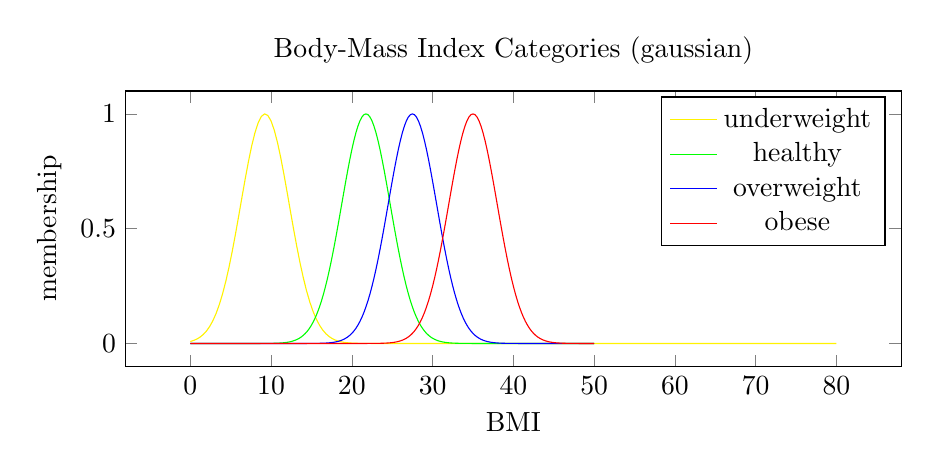
\begin{tikzpicture}
\begin{axis}[
    title=Body-Mass Index Categories (gaussian),
    xlabel=BMI,
    ylabel=membership,
    legend entries={underweight, healthy, overweight, obese},
    width = 4.5in,
    height = 2in
]
\addplot[ % underweight
yellow,
domain=0:80,
samples=201,
]
{exp(-(x-9.25)^2 / 18)};

\addplot[ % healthy
green,
domain=0:50,
samples=201,
]
{exp(-(x-21.75)^2 / 18)};

\addplot[ % overweight
blue,
domain=0:50,
samples=201,
]
{exp(-(x-27.5)^2 / 18)};

\addplot[ % obese
red,
domain=0:50,
samples=201,
]
{exp(-(x-35.0)^2 / 18)};

\end{axis}
\end{tikzpicture}

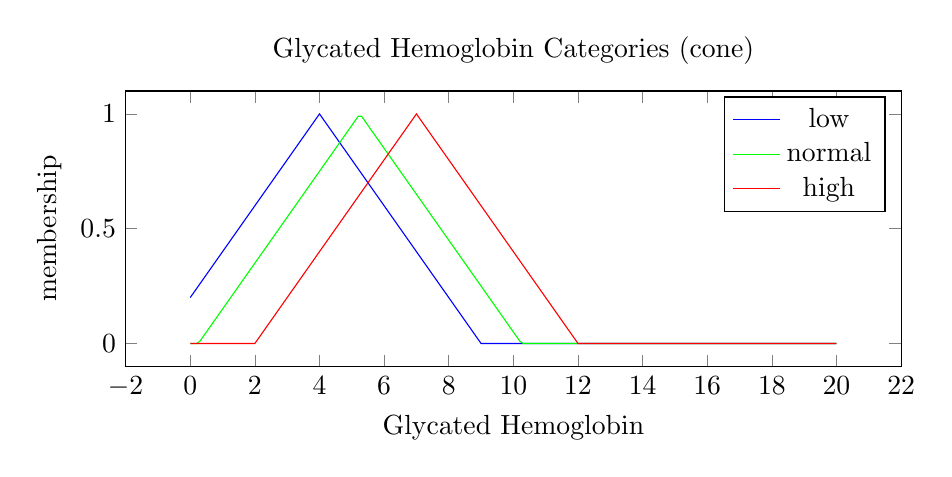
\begin{tikzpicture}[
  declare function={
    cone(\x) = and(\x>=-1,\x<0)*(\x+1) + and(\x>=0,\x<1)*(1-\x);
  }
]
\begin{axis}[
    title=Glycated Hemoglobin Categories (cone),
    xlabel=Glycated Hemoglobin,
    ylabel=membership,
    legend entries={low,normal,high},
    width = 4.5in,
    height = 2in
]
\addplot[ % low
blue,
domain=0:20,
samples=201,
]
{cone((x-4)/5)};

\addplot[ % normal
green,
domain=0:20,
samples=201,
]
{cone((x-5.25)/5)};

\addplot[ % high
red,
domain=0:20,
samples=201,
]
{cone((x-7)/5)};

\end{axis}
\end{tikzpicture}


It should be instructive to see the plots of at least some of
the membership functions, to appeal to our visual intuitions.
Also, for the practical purposes it is inevitable to define the
formulas for the cone and the gaussian curve:

\begin{Verbatim}[samepage=true]
(define ((gaussian center deviation) x)
  (exp (- (/ (square (- x center))
	     (* 2 (square deviation))))))
\end{Verbatim}
\begin{Verbatim}[samepage=true]
(define ((cone center radius) x)
  (cond ((<= x (- center radius))
	 0)
	((<= x center)
	 (/ (+ x (- radius center)) radius))
	((< x (+ center radius))
	 (/ (+ (- x) center radius) radius))
	(else
	 0)))
\end{Verbatim}

In the definition of \texttt{gaussian} we refer to the
built-in exponential function \texttt{(exp x)}, or $e^{x}$.

The definition of the \texttt{cone} function contains
a \texttt{cond} clause that we haven't seen before. It
is actually a variant of the \texttt{if} instruction
that we're already familiar with, and the definition
could as well have been written using the latter form:

\begin{Verbatim}[samepage=true]
(define ((cone center radius) x)
  (if (<= x (- center radius))
    0
    (if (<= x center)
      (/ (+ x (- radius center)) radius)
      (if (< x (+ center radius))
        (/ (+ (- x) center radius) radius)
	0))))
\end{Verbatim}

It is apparent that the form using \texttt{if}
has a more complex structure because of the
higher nesting level.

As all the rules and words' meanings are already known,
the only thing that's left is to actually conduct the
inference: given a tuple of labeled parameters describing
a \texttt{patient}, say, \texttt{((bmi 29) (glycated-hemoglobin 5)
(blood-pressure 20))}, we wish to provide a desired rating for it.
In other words, want to \texttt{(infer \#;from underwriter-rules
\#;about patient \#;within health-categories)}.

First, we need to say to what \texttt{extent} does a
\texttt{patient} belong to a given classes: for example,
according to the membership functions defined above,
the BMI parameter of $29$ may be considered \textit{overweight}
with the degree $0.88$, \textit{obese} with the degree $0.13$,
\textit{healthy} with the degree $0.05$ and \textit{underweight}
with a degree very close to $0$.

So it would be convenient to have a function that, for
a given labeled tuple, returns the extent in which the
tuple's values belong to certain classes defined within
specified categories. It could also be handy if the classes
were sorted, so that the classes to which a given values
``belongs more'' would appear earlier on the list.

\begin{Verbatim}[samepage=true]
(define (extent #;in-which entity #;belongs-to categories)
  (map (lambda ((property value))
	 (let* ((category (lookup property categories))
		(classes (map (lambda ((name extent))
				`(,name ,(extent value)))
			      category)))
	   `(,property . ,(sort classes
				(lambda ((_ degree-1) (_ degree-2))
				  (> degree-1 degree-2))))))
       entity))
\end{Verbatim}
\begin{Verbatim}[samepage=true]
(e.g.
 (extent '((bmi 29) (glycated-hemoglobin 5) (blood-pressure 20))
         health-categories)
 ===> ((bmi (overweight 0.8824969025845955) 
            (obese 0.1353352832366127) 
            (healthy 0.053926197030622854)
            (underweight 3.879522352578383e-10)) 
       (glycated-hemoglobin (normal 0.95) (low 0.8) (high 0.6)) 
       (blood-pressure (overpressure 1.0) 
                       (slight-overpressure 3.3546262790251185e-4) 
                       (high-overpressure 3.3546262790251185e-4)
                       (normal 1.2664165549094176e-14))))
\end{Verbatim}

Probably the most surprising is the use of the \texttt{e.g.} form.
This is a syntactic extension that serves as a lightweight
\textit{unit test} framework: it evaluates the function before
the \texttt{===>} sign and raises an error condition it
its value isn't \texttt{equal?} to the value on the right.
It therefore enhances the reliability of the system, because
we have a confirmation that our function works as expected.

More importantly, it enriches the code with the information that
is more concrete and easier to digest than the sole definition,
because it shows exactly, which outputs can be expected for
given inputs.

The example could not be comprehended in the absence of
the definition of \texttt{health-categories}, but it shows
us what kind of output from the function we should expect,
which in turn prompts us with the idea of how this output
should be processed further.

We ought to take another look at our \texttt{underwriter-rules}.
They all take the form 

\texttt{`(if ,condition (is ,property ,classification))}

where \texttt{condition} either has a form 

\texttt{`(is ,property ,classification)}

or is a junction (i.e. conjunction, disjunction or negation)
of simpler formulas. In the first case, say, 
\texttt{(is bmi overweight)} we evaluate it to the extent
in which the BMI belongs to the set ``overweight''.
In the particular case of BMI being equal $29$, it will
be the value of approx. $0.82$.

In the case of the junction of formulas, we evaluate
it according to the rules given above: conjunction
is the minimum function, disjunction -- the maximum
function, and negation -- the $1-x$ function.
Note the resemblance between the below
\texttt{satisfaction-degree} function and
the definition \texttt{satisfied?} from the earlier chapters.

\begin{Verbatim}[samepage=true]
(define (satisfaction-degree formula interpretation)
  (match formula
    (('and . clauses)
     (minimum (map (lambda (clause)
		       (satisfaction-degree clause interpretation))
		     clauses)))
    (('or . clauses)
     (maximum (map (lambda (clause)
		       (satisfaction-degree clause interpretation))
		     clauses)))
    (('not clause)
     (- 1.0 (satisfaction-degree clause interpretation)))
    (('is property classification)
     (let* ((classifications (lookup property interpretation))
	    ((extent) (lookup classification classifications)))
       extent))))
\end{Verbatim}
\begin{Verbatim}[samepage=true]
;; where
(define (maximum list)
  (match list
    ((last)
     last)
    ((first . rest)
     (max first (maximum rest)))))

(define (minimum list)
  (match list
    ((last)
     last)
    ((first . rest)
     (min first (minimum rest)))))
\end{Verbatim}

We defined two auxiliary functions that designate
the \texttt{minimum} and \texttt{maximum} of the list,
using the built-in \texttt{min} and \texttt{max}
functions that return the largest of its arguments.
As we will see in the following chapters, that definition
wasn't strictly necessary.

Now that we can determine the \texttt{satisfaction-degree}
of a given predicative formula, we have a set of rules
and the preconditions of those rules, the only thing
that is left is to conduct the inference.

This is actually the trickiest part, as it is concerned
with a notion (or rather pseudo-notion) of \textit{defuzzification}.
Let me remind that the \texttt{underwriter-rules} consist
of three rules, corresponding to three possible classifications
of \texttt{rating}: \texttt{standard}, \texttt{perfect} and
\texttt{refuse}. For example, the first rule said:

\begin{Verbatim}[samepage=true]
(if (or (is bmi underweight) (is bmi obese)
        (is glycated-hemoglobin low))
    (is rating refuse))
\end{Verbatim}


We need to blend those three rules, based on the extents
of their preconditions, in order to choose the ``right''
classification.

One idea would be to choose the rule whose precondition
is the highest \texttt{satisfaction-degree}. However, according
to Wikipedia, ``this approach loses information''. Therefore
another method is used: first we clip the membership functions
for the various classes of the category \texttt{rating}, so that
their values are limited to the the satisfaction-degrees, then
we create a new function that gives the maximum of each of the
clipped functions, and finally we apply some numerical method
like calculation of the \textit{center of gravity} of the function
(Wikipedia lists 20 other defuzzification functions, each of them being
equally arbitrary, none of them having any apparent advantages
over the another).

\begin{Verbatim}[samepage=true]
(define (infer #;from rules #;about entity #;within categories)
  (let* ((judgment (extent entity categories)) 
	 (conclusions 
           (map (lambda (('if condition ('is property classification)))
                  (let* ((degree (satisfaction-degree condition judgment))
                         (categories (lookup property categories))
                         ((membership) (lookup classification categories))
                         (conclusion (clip membership 0 degree)))
                    `(,property ,conclusion)))
                rules))
	 (common-subject (equivalence-classes 
			  (lambda ((property-1 _) (property-2 _))
			    (eq? property-1 property-2))
			  conclusions)))
    (map (lambda (((properties functions) ...))
	   (let* (((property . _) properties)
		  (composition (lambda (x)
		 		 (maximum (map (lambda (f) 
                                                 (f x))
                                               functions)))))
	     `(,property ,composition)))
	 common-subject)))
\end{Verbatim}

The code above is somewhat terse, and requires a bit of explanation.
First we calculate the \texttt{judgment} using the \texttt{condition}
function. The \texttt{judgment} therefore contains a list of the
form \texttt{'((bmi (overweight 0.9) (normal 0.1) ...)
(glycated-hemoglobin (normal 0.9) ...) ...)}. Then for each rule
we decompose it into \texttt{condition} and the consequent of the form
\texttt{('is property classification)}, so for example, the name
\texttt{condition} can be bound to the sequence 
\texttt{'(or (is bmi underweight) (is bmi obese) 
(is glycated-hemoglobin low))},  \texttt{property} is bound to 
\texttt{'rating}, and \texttt{classification} is bound to 
\texttt{'refuse}. Then we take the \texttt{membership} function
for the given \texttt{property} and \texttt{classification} pair.
In the case of \texttt{rating}, \texttt{refuse} it is the 
\texttt{(cone 10.0 5.0)} function. Eventually we return a pair with
the name of the classification and the clipped membership function.

Note that although it isn't the case with our example, we could in
general have more properties than just \texttt{rating} contained
in the consequents of our rules. Therefor we would need to split
the rules that refer to the same property. This is what the
\texttt{equivalence-classes} concept is for. In general, it takes
a set and the so-called \textit{equivalence relation}\footnote{
Intuitively, an equivalence relation expresses some sort of common
property, like ``$X$ is of the same religion as $Y$''. This
particular relation divides humans into equivalence classes such
as Buddhists, Christians, Jews, Muslims, and so on, which
leads to many pointless wars.} and returns a list of lists whose
elements all belong to the same equivalence class.

For example, if we had a list of natural numbers, say,
\texttt{(1 2 3 4 5 6 7 8 9)}, then its equivalence classes
for the equivalence relation ``$x$ and $y$ have the same
remainder of the division by $3$'' would be a list of three
lists: \texttt{((1 4 7) (2 5 8) (3 6 9))}.

Although the notion of \texttt{equivalence-classes} isn't essential
for this particular task, it will be used later, so I will present
the code here without any comments, except the note that it preserves
the original order among the elements of the classes, and the
observation that it uses the so-called \textit{named-let} construct
that won't be covered in this pamphlet. The explanation isn't
difficult to find with Google.

\begin{Verbatim}[samepage=true]
(define (equivalence-classes equivalent? set)
  (let next-item ((set set)(result '()))
    (match set
      (()
       (reverse (map reverse result)))
      ((item . set)
       (match result
	 (()
	  (next-item set `((,item) . ,result)))
	 ((this . next)
	  (let next-class ((past '()) (present this) (future next))
	    (match present
	      ((paradigm . _)
	       (if (equivalent? item paradigm)
		   (next-item set `((,item . ,present)
				    . (,@past ,@future)))
		   (match future
		     (()
		      (next-item set `((,item) ,@result)))
		     ((this . next)
		      (next-class `(,present . ,past) this next)))
                    )))
             )))))))
\end{Verbatim}

Having the conclusions split into \texttt{equivalence-classes}
of conclusions that regard the same \texttt{property}, we create
a \texttt{composition} of the clipped functions of \texttt{membership}
to given \texttt{classification}s, which are constructed by
selecting the \texttt{maximum} value of each of the component
functions.

The only thing that may be unknown at this point is what it means
to \texttt{clip} a function. This is rather straightforward:

\begin{Verbatim}[samepage=true]
(define ((clip function bottom top) x)
  (assert (<= bottom top))
  (max bottom (min top (function x))))
\end{Verbatim}

The \texttt{infer} function returns a list of form
\texttt{((property function) ...)}. In order to get
the classifications of the \texttt{property} values,
we need to defuzzify each \texttt{function}.

We are going to use the aforementioned method of
computing the \texttt{center-of-gravity}. This
method is based on \textit{numerical integration}
that will not be covered here.

\begin{Verbatim}[samepage=true]
(with-default ((bottom 0)
	       (top 100)
	       (step 0.1))
  (define (center-of-gravity function)
    (let* ((step (specific step))
	   (domain (range #;from (specific bottom) 
				#;to (specific top) #;by step)))
      (/ (sum (map (lambda (x) (* x (function x) step)) domain))
	 (sum (map (lambda (x) (* (function x) step)) domain))))))
;; where
(define (range #;from bottom #;to top #;by step)
  (if (> bottom top)
    '()
    `(,bottom . ,(range #;from (+ bottom step) #;to top #;by step))))
\end{Verbatim}

The surprising thing is the use of the \texttt{with-default} derived
form. It is used to give some default values to certain names,
but without committing to those values. The form will be explained
in one of the later chapters.

Finally, we can evaluate the expression

\begin{Verbatim}[samepage=true]
(let* ((conclusions (infer #;from underwriter-rules 
				  #;about '((bmi 29) 
					    (glycated-hemoglobin 5) 
					    (blood-pressure 20))
					  #;within health-categories)))
  (map (lambda ((property function))
	 `(,property ,(center-of-gravity function)))
       conclusions))
\end{Verbatim}

to find out that the \texttt{rating} received by our candidate is $7.46$.
In other words, we passed along some numbers to receive yet another number.

\chapter{Matrix Operations}

\begin{chapquote}{David Jacobs}
``Code is like poetry; most of it shouldn't have been written.''
\end{chapquote}

In the previous chapters we've been dealing with certain methods
of \textit{soft computing}. The numerical packages (or ``programming
languages'', as some people call them) like R, SPSS or Matlab
have often been praised for their ``native'' support for matrix
operations and statistical notions.

In this chapter, we will show how easily these concepts can be
implemented in Scheme using the means that we already know. We will
also learn to define and use \textit{variadic} functions.

It is common in mathematics and science to organize the computations
in the form of \textit{matrices}, because this allows to process
large amounts of data in a systematic and uniform manner.

A \textit{matrix} is a rectangular array of numbers, for example

\begin{equation*}
  \begin{pmatrix}
    1 & 2 & 3 & 4 \\
    0 & 4 & 5 & 8 \\
    0 & 0 & 7 & 6
  \end{pmatrix}
\end{equation*}

We can use lists of lists of equal length to represent matrices,
for example

\begin{Verbatim}[samepage=true]
'((1 2 3 4)
  (0 4 5 8)
  (0 0 7 6))
\end{Verbatim}

\subsection{Matrix addition}

Given a matrix, we can determine its \textit{dimensions}.
For example, the above matrix is three-by-four.

\begin{Verbatim}[samepage=true]
(define (dim x)
  (match x
    ((first . rest)
     `(,(length x) . ,(dim first)))
    (_ 
     '())))
\end{Verbatim}

Probably the simplest algebraic operation that one can
conduct on a matrix is \textit{matrix addition}: given
matrices of the same dimensions, we add each element
of one matrix to the corresponding element of the
second matrix:

\begin{Verbatim}[samepage=true]
(define (M+2 A B)
  (assert (equal? (dim A) (dim B)))
  (map (lambda (a b)
	 (map + a b))
       A B))
\end{Verbatim}
\begin{Verbatim}[samepage=true]
(e.g.
 (M+2 '((1 2 3)
        (4 5 6)) '((1 2 3)
                   (4 5 6))) ===> ((2  4  6)
                                   (8 10 12)))
\end{Verbatim}

\subsection{Variadic functions}

I called the function \texttt{M+2} to emphasize that it
takes two arguments. However, because matrix addition is
associative (like conjunction and disjunction in propositional
logic), so it might be more convenient to write
\texttt{(M+ A B C)} instead of \texttt{(M+ (M+ A B) C)}
or \texttt{(M+ A (M+ B C))}. Actually you can check that
this is already the case for scalar addition: the
expression \texttt{(+ 1 2 3)} evaluates to $6$. This
is also true for multiplication.

We can use the \texttt{M+2} function to perform the
generalization to the arbitrary number of arguments,
but no less than one.

\begin{Verbatim}[samepage=true]
(define (M+ . MM)
  (match MM
    ((M)
     M)
    ((A B . X)
     (apply M+ `(,(M+2 A B) . X)))))
\end{Verbatim}

We have used an \textit{improper list} of arguments,
or a \textit{dotted tail notation}. An improper list
is a list whose last \texttt{cdr} is not the empty
list. If the list of arguments is improper, then the
symbol in the dotted tail will be bound the list of
remaining arguments, so for example if we had no
\texttt{list} function defined, we could use that
feature:

\begin{Verbatim}[samepage=true]
(define (list . items)
  items)
\end{Verbatim}
\begin{Verbatim}[samepage=true]
;; or equivalently:
\end{Verbatim}
\begin{Verbatim}[samepage=true]
(define list (lambda items items))
\end{Verbatim}

Note the use of the \texttt{apply} function. It takes
a function and a list of arguments, and \textit{applies}
the function to arguments. For example, if \texttt{l}
is a list containing three elements, then
\texttt{(apply f l)} is equivalent to
\texttt{(f (first l) (second l) (third l))}. However,
if the number of arguments is unknown, then the use
of \texttt{apply} is inevitable if we want to preserve
generality.

Note also, that since the \texttt{max} and \texttt{min}
functions can take the arbitrary number of arguments
(and return the greatest and the smallest of them,
respectively), instead of defining the \texttt{maximum}
and \texttt{minimum} functions, we could have written
\texttt{(apply max ...)} and \texttt{(apply min ...)}.

The \texttt{apply} function can also take a variable
number of arguments -- all arguments between the first
and the last are simply \texttt{cons}ed to the last,
so we could have written \texttt{(apply M+ (M+2 A B) X)}
in the previous definition, yielding the same effect.

\subsection{Transpose}
If we swap columns and rows of a matrix, we obtain
its \textit{transpose}. For example, the transpose
of the matrix
\begin{equation*}
  \begin{pmatrix}
    1 & 2 & 3 \\
    4 & 5 & 6 
  \end{pmatrix}
\end{equation*}
is the matrix
\begin{equation*}
  \begin{pmatrix}
    1 & 4 \\
    2 & 5 \\
    3 & 6
  \end{pmatrix}
\end{equation*}

The code for constructing the transpose of a matrix is
a bit tricky:

\begin{Verbatim}[samepage=true]
(define (transpose M)
  (apply map list M))
\end{Verbatim}

To see why it works, let's try to evaluate
\begin{Verbatim}[samepage=true]
(transpose '((1 2 3)
             (4 5 6)))
\end{Verbatim}

According to our definition, it can be rewritten as

\begin{Verbatim}[samepage=true]
(apply map list '((1 2 3) (4 5 6)))
\end{Verbatim}

which -- according to what we said earlier -- can
be rewritten as

\begin{Verbatim}[samepage=true]
(map list '(1 2 3) '(4 5 6))
\end{Verbatim}

which yields the desired result.

\subsection{Matrix multiplication}

Multiplying two matrices is much trickier than adding
them and is best explained by a math tutor pointing
fingers on the blackboard.

If $A$ and $B$ are matrices, the product $AB$ is
defined only if the number of columns of matrix $A$
equals the number of rows of the matrix $B$. Then,
the number of rows of $AB$ is the same as the number
of rows of $A$, and the number of columns of $AB$
is the same as the number of columns of $B$.

\begin{Verbatim}[samepage=true]
(define (M*2 A B)
  (assert (let* (((A-rows A-cols) (dim A))
		((B-rows B-cols) (dim B)))
            (= A-cols B-rows)))
  (let* ((B^T (transpose B)))
    (map (lambda (rA)
	   (map (lambda (cB)
		  (sum (map * rA cB)))
		B^T))
	 A)))
\end{Verbatim}

We can extend the \texttt{M*2} to support arbitrary
number of arguments analogically as we did for \texttt{M+2}.

There are some other important operations that can be defined
for matrices, like the determinant or rank. Their exposition
is beyond the scope of this pamphlet, but some of them can
be found in this pamphlet's repository.

\chapter{Classifiers}

\begin{chapquote}{Friedrich Nietzsche}
``Truth is a mobile army of metaphors.''
\end{chapquote}

\section{Introduction}

In this chapter, we will be dealing with the task of
\textit{classifying} data -- given a tuple, we need
to classify it to one of given categories, based
on some set of existing classifications (called the
\textit{training set}). We do not know what the
underlying rules of classification are -- our system
should infer that for us.

For the remainder of this chapter, we will be assuming
that a database will be a list of lists, and that
the first list of the database will be a header
(a list of symbol) and all the remaining lists
will contain data, whether it be \textit{numerical} or
\textit{nominal}.

\section{Naive Bayes and Probability}

First of the classifiers that we are going to consider
is based on the notion of \textit{conditional probability}
and makes an indirect use of the so-called
\textit{Bayes theorem}. The underlying idea is very simple:
first we compute the \textit{absolute} probability that
the record belongs to a given class (based on the training
set), then for each possible class we compute the conditional
probabilities of an item of this class having the specified
values as the certain fields of the tuple, multiply it
altogether and choose whichever product of probabilities
turns out to be the greatest. For example, if our data
set has the form

\begin{Verbatim}
(define computer-purchase
  '((age    income student credit-rating buys)
    (31..40 high   no      fair           yes)
    (>40    medium no      fair           yes)
    (>40    high   yes     excellent      yes)
    (>40    low    yes     excellent       no)
    (31..40 low    no      excellent      yes)
    (<=30   medium no      fair            no)
    (<=30   low    yes     fair            no)
   ))
\end{Verbatim}

and we are to predict the class of a new record
\texttt{(>40 low no fair ?)}, then we first compute
the probabilities $P(\mathtt{buys}=\mathtt{yes})$
and $P(\mathtt{buys}=\mathtt{no})$, then we compute
the conditional probabilities 
$P(\mathtt{age}=\mathtt{>40}|\mathtt{buys}=\mathtt{yes})$ and
$P(\mathtt{age}=\mathtt{>40}|\mathtt{buys}=\mathtt{no})$,
the conditional probabilities
$P(\mathtt{income}=\mathtt{low}|\mathtt{buys}=\mathtt{yes})$ and
$P(\mathtt{income}=\mathtt{low}|\mathtt{buys}=\mathtt{no})$,
and so on (for all the other data). For example, for this particular
database, $P(\mathtt{buys}=\mathtt{yes})$ is $\frac{4}{7}$,
because there are $7$ entries, and $4$ of them have
the \texttt{buys} field equal to \texttt{yes}. Similarly,
$P(\mathtt{age}=\mathtt{>40}|\mathtt{buys}=\mathtt{yes})$
equals $\frac{2}{4}$, because there are $4$ entries that have
the \texttt{buys} field equal to \texttt{yes}, and $2$ of them
have the \texttt{age} field equal to \texttt{>40}.

Note that, unlike in the case of fuzzy logic, the values
of probabilities have a well-defined meaning, so we shouldn't
be disgusted with this approach, at least not in principle.

Having computed the conditional probabilities for both
\texttt{buys}=\texttt{yes} and \texttt{buys}=\texttt{no},
we multiply them by the corresponding probabilities of
belonging to given \texttt{buys} classes and choose the
class whose probability is higher.

\subsection{What is the universe}

We have used the notation that is commonly used in the
mathematics: $P(\phi)$ is a probability that the
proposition $\phi$ is satisfied, and $P(\phi|\psi_1,...,psi_n)$
is a probability that the proposition $\phi$ is
satisfied given that $\psi_1,...,psi_n$ are satisfied.

The exact meaning of the proposition is usually relative
to some context or situation (in this case -- our database).
In the remainder of this pamphlet, we will be referring to
this situation as \texttt{universe}.

In our case, the structure of a \texttt{universe} is rather
simple and can be divided into two realms: the realm of
\textit{ideas} and the realm of \textit{entities}. The
realm of ideas names the possible properties of each
single entity, and each entity consists of values whose
meaning is specified in the realm of ideas. The variable
\texttt{computer-purchase} is an example of a universe: the first
element of the list is the realm of ideas, and contains
the names of $5$ properties: \texttt{(age income student
credit-rating buys)}. The rest of the lists contains $7$
individual entities, each of them obviously having $5$
properties.

We may wish to refer to the property of an entity
from the specific universe, for example \textit{the age
of a person}. For this purpose, we will define the
function \texttt{the}:

\begin{Verbatim}[samepage=true]
(with-default ((universe '(()())))
  (define (the property #;of item)
    (let* (((names . things) (specific universe))
	   (index (list-index (lambda (label) 
                                (eq? label property)) 
                              names)))
      (if (not index)
	  (throw 'not-found property names))
      (list-ref item index))))
\end{Verbatim}

We have used the \texttt{with-default} derived form
that we have also used in the definition of the
\texttt{center-of-gravity} function that was used
in the defuzzification process. The default universe
consists of an empty realm of ideas and of a single
entity with no properties.

Unlike the \texttt{center-of-gravity} function,
the default context of the \texttt{the} function isn't
particularly helpful, so we will likely need to
override the desired value somehow. For this purpose,
we will use another derived form called \texttt{specify}.

For example, the expression
\begin{Verbatim}[samepage=true]
(specify ((universe '((name age))))
  (the 'age #;of '(George 48)))
\end{Verbatim}
evaluates to \texttt{48}.

If we wanted to express the naive Bayes classifier,
we'd need to use the notion of \texttt{probability}.
The proposition in the form $P(\phi)$ can be expressed
using regular functions (i.e. lambdas) ranging the
objects in the universe, for example
$P(\mathtt{buys}=\mathtt{yes})$ could be paraphrased as
\begin{Verbatim}[samepage=true]
(probability 
  (lambda (item) 
    (eq? (the 'buys item) 'yes)))
\end{Verbatim}

Likewise, we could define \texttt{probability} as
a variadic function, treating all the additional
arguments as the \textit{given} propositions:

\begin{Verbatim}[samepage=true]
(with-default ((universe '(()())))
  (define (probability proposition #;given . circumstances)
    (let* (((names . things) (specific universe))
	   (known-world (filter (apply compose circumstances) 
				things)))
      (/ (count proposition known-world)
	 (length known-world)))))
\end{Verbatim}

where \texttt{compose} is a function that takes arbitrary
number of functions and returns their \textit{composition}
(if there are no arguments, the \textit{identity} function
is returned), i.e. \texttt{((compose f g) x)} means the
same as \texttt{(f (g x))}.

Back to the Naive Bayes classifier, we can stick to
the convention that the unknown property (whose value
is supposed to be used) will be represented using the
question mark symbol. Therefore we expect that the

\begin{Verbatim}[samepage=true]
(specify ((universe computer-purchase))
  (naive-bayes '(>40 low no fair ?)))
\end{Verbatim}

will try to classify the last entry in the tuple, i.e.
the \texttt{buys} property. Therefore we may need to be able
to retrieve the name of the unknown property, as well
as the names of the known properties (note that we assume
that there's only one unknown per tuple):

\begin{Verbatim}[samepage=true]
(without-default ((universe '(()()))
                  (unknown? (lambda (x) (eq? x '?))))
  (define (unknown-label+rest tuple)
    (let* (((header . data) (specific universe))
	   (unknown/index (list-index (specific unknown?) tuple))
	   (unknown-property (list-ref header unknown/index))
	   (known-properties (filter (lambda (label)
				       (not (eq? label unknown-property)))
				     header)))
      (values unknown-property known-properties))))
\end{Verbatim}

The novel thing is the use of the function \texttt{values}.
One of the most controversial features of Scheme is the functions'
ability to have more than one value. It is useful on some
occasions though, because it allows to extend a function
to give additional information without breaking any existing
code. It may be considered inelegant though, and perhaps
it would be better to define two functions rather than one.


In addition to retrieving the name of the unknown, it would 
also be helpful if we were able to get all the possible values
of a given property within a universe, in order to compute
the appropriate conditional and unconditional probabilities:

\begin{Verbatim}[samepage=true]
(with-default ((universe '(()())))
  (define (column name)
    (let* (((header . data) (specific universe))
	   (index (list-index (lambda (x) (eq? x name)) header)))
      (map (lambda (row)
	     (list-ref row index))
	   data)))

  (define (possible-values attribute)
    (delete-duplicates (column attribute))))
\end{Verbatim}
\begin{Verbatim}[samepage=true]
(e.g.
 (specify ((universe computer-purchase))
   (possible-values 'age)) ===> (<=30 31..40 >40))
\end{Verbatim}

Note that we also defined a \texttt{column} auxiliary function
that allows us to project the universe onto one of its dimensions.
That function will also be used later.

We can now define the Naive Bayes of a record in the following way:

\begin{Verbatim}[samepage=true]
(with-default ((universe '(()())))
  (define (naive-bayes tuple)
    (let* ((unknown-property known-properties 
			     (unknown-label+rest tuple))
	   (classes (possible-values unknown-property)))

      (define (unconditional-probability class)
        (probability (lambda (x) 
                        (eq? (the unknown-property x) class))))

      (define (partial-conditional-probabilities #;for class)
	(map (lambda (property)
               (probability 
                 (lambda (item)
		   (eq? (the property item) (the property tuple)))
		 #;given
		 (lambda (item)
		   (eq? (the unknown-property item) class))))
	      known-properties))

      (apply argmax (lambda (class)
                      (apply * (unconditional-probability class)
                               (partial-conditional-probabilities
                                class)))
              classes))))
\end{Verbatim}

In the definition, we introduced two auxiliary definitions
of \texttt{unconditional-probability} of belonging to a \texttt{class}
and of \texttt{partial-conditional-probabilities} of having
certain properties given that we belong to given \texttt{class}.

We have also used the \texttt{argmax} library function that
takes a measure function and arbitrary number of arguments
and returns the argument whose measure is the greatest.

The code above expresses the idea of the naive Bayesian
classifier in a manner that is probably a lot more precise
and concise than the textual description given at the
beginning of this section. It may take some time to be able
to both read and write such code, but once it is mastered,
it becomes as natural as listening and talking, allowing to
express more and more advanced concepts.
\section{Decision Trees and Information}

The naive Bayes classifier is structurally very simple.
In this section we are going to learn about a slightly
more sophisticated classifier known as the \textit{decision
tree}. It is interesting, because in addition to being
a classifier, it can also be seen as an algorithm for
compressing knowledge contained in a data set.

In general, a decision tree is an acyclic directed graph
whose nodes alternately represent questions and possible
answers to those questions. Usually there are many ways
in which a decision tree can be constructed for a given
data set, but some of those graphs are more compact than
others (i.e. contain less nodes). In the worst case the
number of leaves in a tree can be equal to the number
of database entries. This can depend on both the structure
of data and on the order in which we decide to ask questions,
so it is important to ask them in a way that allows to
reject as many alternative options as possible.

For example, let's take a look at this slightly larger version
of the \texttt{computer-purchase} database:
\begin{Verbatim}
(define computer-purchase
  '((age     income student credit-rating buys)
    (<=30    high   no      fair            no)
    (<=30    high   no      excellent       no)
    (31...40 high   no      fair           yes)
    (>40     medium no      fair           yes)
    (>40     low    yes     fair           yes)
    (>40     low    yes     excellent       no)
    (31...40 low    yes     excellent      yes)
    (<=30    medium no      fair            no)
    (<=30    low    yes     fair           yes)
    (>40     medium yes     fair           yes)
    (<=30    medium yes     excellent      yes)
    (31...40 medium no      excellent      yes)
    (31...40 high   yes     fair           yes)
    (>40     medium no      excellent       no)
   ))
\end{Verbatim}

We can notice, that if a person's \texttt{age} is \texttt{<=30},
then that person buys a computer only if she or he is a student
-- thus we can get the answer after two questions. People whose
\texttt{age} is \texttt{31...40} always buy a computer. If
a person's \texttt{age} is \texttt{>40}, then he or she buys
a computer only if the \texttt{credit-rating} is \texttt{fair}.

The above \textit{decision process} can be represented
in the form of a tree:
\begin{center}
\Tree [.age 
  [.<=30 
    [.student 
      [.no no ]  
      [.yes yes ]  ]  ]  
  [.31...40 yes ]  
  [.>40 
    [.credit-rating 
      [.fair yes ]  
      [.excellent no ]  ]  ]  ]
\end{center}

\subsection{Representing trees in Scheme}

One could ask how can we represent such a tree in Scheme.
The truth is however that we already have, by using nested
lists. The most straightforward way of representing a binary
tree with labeled nodes is to use a list of the form
\texttt{(label branches ...)}, where \texttt{branches}
are also trees. The only exception is that we represent
leaves as atomic objects. So for example, the above
tree could be written as the following Scheme expression:
\begin{Verbatim}[samepage=true]
(age (<=30 (student (no no)
                    (yes yes)))
     (31...40 yes)
     (>40 (credit-rating (fair yes)
                         (excellent no))))
\end{Verbatim}

It may not be immediately apparent that those two objects
are \textit{isomorphic}, and besides the former is much more
pleasant to watch, so it would be helpful if we could convert
Scheme expressions to pictures in a systematic way. This shouldn't
be particularly difficult -- the above tree was generated
in \LaTeX{} using the \textit{qtree} package from the following
code:
\begin{Verbatim}[samepage=true]
\Tree [.age 
  [.<=30 
    [.student 
      [.no no ]  
      [.yes yes ]  ]  ]  
  [.31...40 yes ]  
  [.>40 
    [.credit-rating 
      [.fair yes ]  
      [.excellent no ]  ]  ]  ]
\end{Verbatim}

(Note the resemblance). Before we create our converter, however,
we should note one thing: although for simple examples such as
the one above we could decide, for a given path on the tree,
which label should be assigned to a given data tuple, our
database could contain a few tuples with the same values but
different labels, like:

\begin{Verbatim}[samepage=true]
  ...
  (<=30 high no fair no)
  ...
  (<=30 high no fair yes)
  ...
\end{Verbatim}

In such situations, we would rather that the leaf contained
the \textit{probability distribution} of belonging to certain
classes, than a single value. How do we do that, if we already
used pairs to represent trees?

One way would be to change our representation of a tree, so
that the nodes, branches or leaves were tagged somehow.
However that would add complexity (and perhaps ambiguity)
to our representation.

Another way would be to \textit{freeze} compound data structures
so that they could be seen as atomic objects in the context
of a tree, but could also be \textit{defrost} for further
processing.

Scheme does provide some means for freezing the compound
objects: in addition to lists or pairs, one can also use
containers called \textit{vectors}, and convert vectors
to lists and lists to vectors using \texttt{vector->list}
and \texttt{list->vector} built-in procedures.

We can therefore assume that a leaf of a tree is either
a symbol or a vector, and in the latter case we would
like to generate a table containing the information from
that vector. The probability table will have the form

\begin{Verbatim}[samepage=true]
#((class-1 probability-1)
  (class-2 probability-2)
  ...)
\end{Verbatim}

where \texttt{\#(elements ...)} is a legitimate Scheme
notation for vectors.

The code for converting Scheme objects to \LaTeX{} trees
and tabulars looks as follows:

\begin{Verbatim}[samepage=true]
(define (latex/tabular rows)
  (let* ((columns (length (first rows))))
    (string-append
     "\\begin{tabular}{"
     (string-join (make-list columns "c") "")
     "} "
     (string-join 
      (map (lambda (row)
	     (string-join (map ->string row) " "))
	   rows)
      " \\\\ \\hline ")
     " \\end{tabular}")))
\end{Verbatim}
\begin{Verbatim}[samepage=true]
(define (latex/qbranch tree)
  (match tree
    ((node . branches)
     (string-append 
      "[." (->string node) " "
      (string-join (map latex/qbranch branches) " ")
      " ] "))
    ((? vector?)
     (string-append 
      "\n[.{"
      (latex/tabular (vector->list tree))
      "} ] "))
    (leaf
     (->string leaf))))
\end{Verbatim}
\begin{Verbatim}[samepage=true]
(define (latex/qtree tree)
 (string-append 
  "\\begin{figure}"
  "\\Tree "
  (latex/qbranch tree)
  "\\end{figure}"))
\end{Verbatim}

The \texttt{latex/qtree} interface is a simple wrapper on the
\texttt{latex/qbranch} function that ``does all the work'', i.e.
that converts a tree into a string containing \LaTeX{} code
for displaying a tree. The \texttt{latex/tabular} function
does nothing beyond the obvious.

The defined functions make an extensive use of built-in functions
\texttt{string-append} and \texttt{string-join} as well as
a library function \texttt{->string} that converts arbitrary
Scheme objects to strings.

Note that we had to escape the slash symbols for \LaTeX{}.

\subsection{Constructing a decision tree}

Now that we are equipped with proper tools for visualizing
the tree structures, we can try to construct a tree for
a given data set. In order to do so, let's recall the informal
construction of the tree that we conducted at the beginning
of this section. The first question that we chose to divide
our set was about the \texttt{age}, because it seemed
intuitive that this parameter was most \textit{informative}
with regard to the question whether a given person \texttt{buys}
a computer or not.

Regardless of the underlying intuitions, we can show how to
construct a decision tree, provided that we know how to
specify what is an \texttt{information-gain} of an
\texttt{attribute} with regard to a certain \texttt{label}
(which, in the above case, is the \texttt{buys} attribute).

The construction for a given database will proceed by
splitting the database rows into equivalence classes
according to the values of the considered attributes,
and removing the columns containing the attributes that
have already been considered. The smaller databases
created in this way will be called \texttt{slices}:

\begin{Verbatim}[samepage=true]
(define (drop-column database label)
  (let* (((header . data) database)
	 (index (list-index (lambda (name) (eq? name label)) header)))
    (map (lambda (row)
	   (skip index row))
	 database)))
\end{Verbatim}
\begin{Verbatim}[samepage=true]
(define (slices #;of database #;on attribute)
  (specify ((universe database))
    (let* (((names . things) database)
           (classes (possible-values attribute)))
      (values
       (map (lambda (class)
              (let* ((peers (filter (lambda (item)
                                      (eq? (the attribute item)
                                           class))
                                    things)))
                (drop-column `(,names . ,peers) attribute)))
            classes)
       classes))))
\end{Verbatim}

The \texttt{(skip i l)} is a library function that returns a copy
of list \texttt{l} without its \texttt{i}-th element.

The construction stops (for a given slice) either when
every record of that slice has the same value of the \texttt{label}
attribute (e.g. \texttt{buys}=\texttt{yes}), or when the
only column left in the database is the \texttt{label} -- in
the former case we know what the node value should be, but in
the latter we need to construct the probability distribution
table:

\begin{Verbatim}[samepage=true]
(define (probability-table ((label) . column))
  (specify ((universe `((,label) . ,column)))
    (let* ((classes (possible-values label)))
      (map (lambda (class)
	     `(,class ,(probability (lambda (item)
				      (eq? (the label item)
					   class)))))
	   classes))))
\end{Verbatim}
\begin{Verbatim}[samepage=true]
(define (decision-tree #;of data #;for label)
  (match data
    (((last) . _)
     (assert (eq? label last))
     (list->vector (probability-table data)))
    ((names . things)
     (let* ((attributes (filter (lambda (name)
                                  (not (eq? name label)))
                                names))
            (attribute (apply argmax
                              (lambda (attribute)
                                (specify ((universe data))
                                  (information-gain attribute label)))
                              attributes))
            (sections classes (slices #;of data #;on attribute))
            (branches (map (lambda (class section)
                             (specify ((universe section))
                               (match (possible-values label)
                                 ((result)
                                  `(,class ,result))
                                 (_
                                 `(,class ,(decision-tree section
                                                          label))))))
                           classes sections)))
       `(,attribute . ,branches)))))
\end{Verbatim}

What's left before our code can actually work is to define
the \texttt{information-gain} somehow. There are many ways
in which it can be defined. I will present the definition
based on Claude Shannon's notion of \textit{information entropy},
although I need to note that I do not comprehend it fully.

We start off by defining the measure of information
contribution of given proposition:

\begin{Verbatim}[samepage=true]
(define (information proposition #;given . circumstances)
  (let ((p (apply probability proposition circumstances)))
    (if (zero? p)
        0.0
        (- (* p (log p))))))
\end{Verbatim}

As we can see, the notion of \textit{information} is defined
in terms of \texttt{probability}, so it needs a specific
\texttt{universe} to operate on. It also allows to specify
``conditional information'', which corresponds exactly to
the conditional probability.

We had to check whether the probability of given event is
zero, because if it were, then the logarithm of that probability
would be $-\infty$, and in the Scheme arithmetic zero times
$\infty$ is not a number.

The notion of \texttt{information} is used in the definition
of \texttt{information-gain}:

\begin{Verbatim}[samepage=true]
(define (information-gain attribute target-class)
  (let* ((classes (possible-values target-class)))
    (- (sum (map (lambda (class)
                   (information (lambda (item)
				  (eq? (the target-class item)
				       class))))
		 classes))
	 (attribute-entropy attribute target-class))))
\end{Verbatim}
\begin{Verbatim}[samepage=true]
;; where
(define (attribute-entropy attribute target-class)
  (let* ((classes (possible-values target-class))
         (options (possible-values attribute)))
    (sum (map (lambda (option)
                (sum (map (lambda (class)
			    (* (information
			        (lambda (item)
                                  (eq? (the target-class item)
				       class))
			        #;given
			        (lambda (item)
                                  (eq? (the attribute item)
				     option)))
			       (probability
			        (lambda (item)
				  (eq? (the attribute item)
				        option)))))
			  classes)))
	      options))))
\end{Verbatim}
The definitions are rather simple structurally, and the
only problem with their comprehension may stem from the
lack of understanding of the underlying theory.

\subsection{Deciding upon a decision tree}

Now that we know how to build trees, we may wish to use
them as classifiers: we shall follow the tree according
to the path specified by the properties of the data that
we wish to classify. If the leaf that we reached is
a single value, we simply assign it to our tuple.
Otherwise it is a probability distribution table, and
we should draw lots according to that distribution:

\begin{Verbatim}[samepage=true]
(define (draw-lots probability-table)
  (let* ((((classes probabilities) ...) probability-table)
	 (cumulative-distribution (scan + 0 probabilities))
	 (lot (random 1.0))
	 ((class upper-limit) (find (lambda ((class upper-limit))
				      (<= lot upper-limit))
				    (zip classes 
					 cumulative-distribution))))
    class))
\end{Verbatim}

we used here the \texttt{scan} library function for calculating
\textit{prefix sum}. Assuming that \texttt{(random 1.0)} returns
an evenly distributed random variable, this method is known
as \textit{inverse transform sampling}.

The code for actually making a decision based on the tree
isn't particularly complicated.
\begin{Verbatim}[samepage=true]
(with-default ((universe '(()())))

  (define (decide/tree tuple)
    (let* ((unknown-label (unknown-label+rest tuple))
	   (tree (decision-tree (specific universe) unknown-label)))
      (tree-decide tree tuple)))
  
   (define (tree-decide tree tuple)
     (match tree
       ((property . selections)
	(let* ((class (the property tuple))
	       ((_ next) (find (lambda ((value next)) 
		                 (eq? value class)) 
			       selections)))
	  (tree-decide next tuple)))
       ((? vector? probability-table)
	(draw-lots probability-table))
       (_
	tree))))
\end{Verbatim}
The \texttt{decide/tree} procedure constructs a tree for the
unknown label, and then refers to the \texttt{tree-decide}
function that actually traverses the path on the tree by
recursively calling itself. The code follows the established
convention of operating within the context of \texttt{universe}.

\section{k Nearest Neighbours}

So far we have been dealing with a \textit{nominal} database,
i.e. such that its entries belonged to a finite set of
unordered values. In this section, we are going to learn
about the \textit{k Nearest Neighbours} classifier that
is intended to handle the \textit{numerical} data, i.e.
data consisting of real numbers.

For this purpose, we will use the database acquired from
\textit{The Data-mining Project} called ``iris.csv'', which
-- as its name suggests -- is stored in a CSV file.

Although the format is rather simple (it is a simple line-based
text file), there is a readily available library for Guile
(surprisingly called ``Guile-CSV'') that we will use for reading
the data. The patched version of the library (with a simplified
interface) is available in the pamphlet's repository, as well
as the database itself.

In order to load the ``iris.csv'' database, having loaded
the \texttt{(guile csv)} module, we shall write 

\texttt{(define iris (read-csv "iris.csv"))}

The database is compatible with previously described structure
of the \texttt{universe}. All columns but the last contain
some numerical data (dimensions of certain parts of flowers),
while the last column, labeled as \texttt{class}, contains
the name of the flower species: \texttt{Iris-setosa},
\texttt{Iris-versicolor} or \texttt{Iris-virginica}.

The numerical parameters of database entries can be seen
as points in a multi-dimensional space. The idea behind
the \textit{k Nearest Neighbours} classifier is simple:
given a point that we wish to classify, we take a look
at the $k$ nearest existing points, and classify the new
point to the class to which the majority of those nearest
points belongs.

We will be assuming, that in the given data set
the classification is always the last field. While
this may not be the most fortunate idea in general,
it turned out to be sufficiently good in practice
(it is always OK to generalize the code when needed).

In order to build the desired classifier, we actually
only need only three functions: one that would allow
us to compute the \textit{distance} between two points,
another for finding the nearest neighbours and one for
taking the majority of them.

With regard to the distance, we will be using the
\texttt{euclid-distance} function:

\begin{Verbatim}[samepage=true]
(define (euclid-distance a b)
  (sqrt (sum (map square (map - a b)))))
\end{Verbatim}

Note that -- in addition to the built-in \texttt{sqrt} function
for computing the square root of a number, we have used two
functions defined in the first chapter. How surprising the
life can be!

Also note, that the function makes no assumptions on the
dimensionality of the space that we investigate.

In the case of the \texttt{nearest-neighbours} procedure,
we will simply sort the data according to the distance between
its points and the point being classified, and then we take
the $k$ first points from the list. For the practical reasons,
we will compute the distance and attach that information to
database before sorting -- that way we will avoid computing
the value of the distance function in each comparison.

\begin{Verbatim}[samepage=true]
(define ((nearest-neighbours k #;in data) #;of sample)
  (let* ((measured (map (lambda ((values ... label))
			  `(,(euclid-distance values sample) 
			    ,@values ,label))
			data))
	 (sorted+ (sort measured
			(lambda ((distance-1 . _) (distance-2 . _))
			  (< distance-1 distance-2))))
	 (sorted (map (lambda ((distance . data)) data) sorted+)))
    (take sorted k)))
\end{Verbatim}

Lastly, we need to choose the label such that the majority
of the points bear it. We will use the \texttt{equivalence-classes}
operation to facilitate that:

\begin{Verbatim}[samepage=true]
(define (dominant-label labeled-points)
  (let* ((classes (equivalence-classes
                   (lambda ((_ ... label-1) (_ ... label-2))
                     (eq? label-1 label-2))
                   labeled-points))
         (biggest (apply argmax length classes))
         (((_ ... label) . _) biggest))
    label))
\end{Verbatim}

The only thing that's left is to bring those ideas together:

\begin{Verbatim}[samepage=true]
(define (((classify/knn k) universe) sample)
  (let* (((header . data) universe))
    (dominant-label ((nearest-neighbours k data) sample))))
\end{Verbatim}

\section{Quantization of numerical data}

Suppose that we want to classify numerical data using
our decision trees or naive Bayes classifier. Applying them
to numerical data could be rather inefficient, because we
would likely obtain very low probabilities in the naive
Bayes classifier, and very complex and inaccurate decision
trees (and most likely no path on the decision tree would
correspond to our data).

A possible solution would be to split the numerical data
into intervals, and construct trees or compute probabilities
for those intervals, rather than exact numbers. This method
is called \textit{quantization}. In particular, if all 
the intervals (except, perhaps, the first and the last one)
are of the same length, then we deal with \textit{uniform
quantization}\footnote{Perhaps a more fruitful idea would
be to quantize the data so that the number of elements
that belong to various intervals is equal, rather than
the length of the intervals.}.

This section presents briefly how the numerical data
can be quantized.

The procedure is rather straightforward -- for each
dimension, we need to take the extreme values (the
lowest and the highest). They will span over the range
that will be used for quantization. Additional categories
will be created for points lying beyond those extremes.

In order to classify a point, we search all the intervals
and return the one the given point belongs to.

We need to classify each dimension separately, so we
shall create a list of \textit{quantizers} (i.e. functions
that assign a point the name of its range).

This is how this works in practice:

\begin{Verbatim}[samepage=true]
(with-default ((intervals 5)
	       (universe '(()())))
  (define ((quantizer label) value)
    (let* ((data (column label))
	   (low high (apply min+max data))
	   (unit (/ (- high low) (specific intervals)))
	   (range (iota (specific intervals) low unit))
	   (upper-bound (find (lambda (upper-bound)
				(< value upper-bound))
			      range)))
      (if upper-bound
	  (symbol-append '< (number->symbol upper-bound))
	  (symbol-append '>= (number->symbol high)))))

  (define (quantize-item)
    (let* ((((header ... class) . _) (specific universe))
	   (quantizers (map quantizer header)))
      (lambda ((values ... label))
	`(,@(map (lambda (quantize value) 
		   (quantize value))
		 quantizers values) ,label)))))
\end{Verbatim}
\begin{Verbatim}[samepage=true]
(define (quantize universe)
  (let (((header . data) universe))
    (specify ((universe universe))
      `(,header . ,(map (quantize-item) data)))))
\end{Verbatim}

For creating the names of the labels, we have used library
functions \texttt{symbol-append} and \texttt{number->symbol},
whose names are rather self-explanatory. As you can see,
we only use the upper-bounds to name the intervals, so for
example if we want to classify number $21.5$ to one of intervals
 $(-\infty, 18.0]$, $(20.0, 22.0]$, $(22.0, 24.0]$, $(24.0, +\infty)$,
it will be labeled as \texttt{<22.0}.

Of course, we need to create a quantized version of a universe
in order to further operate on it, for example:

\begin{Verbatim}[samepage=true]
(define iris/quantized (quantize iris))
\end{Verbatim}

\section{Evaluating classifiers}

Although we have presented a few methods for classifying data,
it would be interesting to ask whether they actually work, or
to what extent we can rely on them. This section will present
a small framework for evaluating the classifiers.

The idea is to divide our data set into two parts:
the \textit{training} part (that would be the base for the
construction of decision trees, calculating Bayesian probabilities,
or determining the set of neighbours that we use for classification)
and the \textit{verification} part that would allow us to
determine how many predictions were right and in how many cases
our classifier was mistaken, and what sort of errors it made.

In order to do so, we shall write a procedure that takes
a given strategy (understood as a function that takes the
training set and produces a function that actually performs
classification of samples), a training/verification set and
a fraction that expresses how big should be the training set
compared to verification set, and returns some detailed
information regarding the confusions made.

\begin{Verbatim}[samepage=true]
(define (evaluate-strategy strategy training-proportion data)
  (assert (< 0 training-proportion 1))
  (let* (((header . data) data)
	 (classes (equivalence-classes 
		   (lambda ((_ ... label-1) (_ ... label-2))
		     (eq? label-1 label-2))
		   data))
	 (((training . verify) ...)
	  (map (lambda (class)
		 (let* ((total-size (length class))
			(training-size (inexact->exact 
					(floor (* training-proportion
						  total-size))))
			(training verify (split-at class 
						   training-size)))
		   `(,training . ,verify)))
	       classes))
	 (training verify (values `(,header . ,(concatenate training))
				  (concatenate verify)))
	 (classify (strategy training))
	 (classified (map (lambda ((sample ... label))
			    `(,(classify sample) . ,label))
			  verify)))
    (values
     (confusion-matrix classified)
     (exact->inexact (/ (count (lambda ((guess . real))
				 (not (eq? guess real)))
			       classified)
			(length classified))))))
\end{Verbatim}

Despite its length, the code is rather simple. The only new
thing here is the use of the library function \texttt{concatenate}
that takes a list of lists and returns a list of elements of
those lists, for example \texttt{(concatenate '((1 2) '(3) '(4 5)))}
would return a list \texttt{(1 2 3 4 5)}, and the use of the
\texttt{inexact->exact} procedure, that requires a bit of
explanation. The Scheme programming language has two distinct
types of numbers: exact, which include integers and rationals,
and inexact, that correspond to the notion of \textit{floating
point} numbers\footnote{Actually, the notion of inexact numbers
also embraces \textit{complex numbers} that are represented
as pairs of floating point numbers.}. The exact numbers are called
so because they can be arbitrarily large (with regard to integers)
or arbitrarily small (with regard to fractions), while the
inexact numbers are always represented with limited precision.
The above use of the \texttt{inexact->exact} function stems from
the fact that for some reason the \texttt{floor} function
(which returns the largest integer part of its argument)
returns an inexact number, while the \texttt{split-at} function
takes an exact.

The most important thing that the \texttt{evaluate-strategy}
function does is producing a pair of labels \texttt{(guess . real)}
based on the verification set and gathering them in the
\texttt{classified} list. Then the list is passed on to the
\texttt{confusion-matrix} procedure that makes a summary of
errors:

\begin{Verbatim}[samepage=true]
(define (confusion-matrix classified-data)
  (let* ((rows (equivalence-classes (lambda ((a . _)(b . _))
				      (eq? a b))
				    classified-data)))
    (map (lambda (row)
	   (let* ((classes (equivalence-classes
			    (lambda ((_ . a) (_ . b))
			      (eq? a b))
			    row))
		  (total (length row)))
	     (map (lambda (class)
		    (let* ((((labeled . guessed) . _) class)
			  (classified (length class)))
		      `(,labeled ,guessed ,classified ,total 
				 ,(exact->inexact 
				   (/ classified total)))))
		  classes)))
	 rows)))
\end{Verbatim}

As we said earlier, the use of the evaluator requires us
to stick to certain conventions -- the strategy needs to
be a function that takes data and returns a classifier
for a single sample. The \texttt{classify/knn} function
already conforms to that convention (once the \texttt{k}
is settled), but the other two classifiers do not, and
therefore we need to adopt them:
\begin{Verbatim}[samepage=true]
(define ((classify/naive-bayes data) sample)
  (specify ((universe data))
    (naive-bayes `(,@sample ?))))
\end{Verbatim}
\begin{Verbatim}[samepage=true]
(define ((classify/decision-tree data) sample)
  (specify ((universe data))
    (let* ((tree (decision-tree data 'class)))
      (tree-decide tree sample))))
\end{Verbatim}

Note that the \texttt{classify/decision-tree} will
misbehave under the substitutional model of computation,
because it will require to reconstruct the decision tree
for each sample. This can be solved easily using the
technique of \textit{memoization} that we will not cover
here.

Finally, we can use our evaluator to verify the quality
of our classifiers:

\begin{Verbatim}
(evaluate-strategy classify/decision-tree 7/10 iris/quantized)
\end{Verbatim}

\section{Clusterization}
In the previous sections we've been dealing with a task
of assigning known labels to the elements in a set. This
section presents a method called \textit{k means} that
allows to established distinct categories within an unlabeled
set of numerical data. This technique is in general called
\textit{clusterization}.

Although it may sound fancy, the method of $k$ means is
rather simple, but also limited, because it requires its
user to provide the maximum number of clusters that are
to be found in the set.

Once it is done, we choose random points in a given space
and for each of those points, we assign it the samples that
are the nearest. Then we replace the random points with
mean values of those samples, and repeat that process
until we reach a \textit{fixed point}, i.e. until the
points remain the mean values of the attracted samples.

In order to pick the random values, we first need to
specify the ranges among which we ought to choose, so
that we can select a value from within that range.
Then, we simply generate a list of points of the desired
length:

\begin{Verbatim}[samepage=true]
(define (random-centers k data)
  (let* ((upper (apply map max data))
	 (lower (apply map min data)))
    (generate-list k (lambda ()
		       (map (lambda (lower upper)
			      (+ lower (random (- upper lower))))
			    lower
			    upper)))))
\end{Verbatim}

Once you get used to using \texttt{map}, \texttt{apply} and
\texttt{lambda}, the code is very straightforward and needs
no comment. Before this happens, you probably need to practice
a lot, though.

The assignment of samples to the alleged cluster centers
is also very simple, once you get familiar with the notion
of \texttt{equivalence-classes}:

\begin{Verbatim}[samepage=true]
(define (classify data centroids)
  (let* ((nearest-centroid (lambda (point)
			     (apply argmin 
                                    (lambda  (c) 
                                      (euclid-distance point c))
				    centroids)))
	 (clusters (equivalence-classes 
                     (lambda (a b)
	               (equal? (nearest-centroid a)
			       (nearest-centroid b)))
		    data)))
    clusters))
\end{Verbatim}

When we put those two above together, we get the
clusterization routine:

\begin{Verbatim}[samepage=true]
(define (clusterize data k)
  (let* ((centroids (random-centers k data))
         (clusters (classify data centroids))
	 (new-centroids (map (lambda (cluster)
			       (apply map (lambda elements 
					    (mean elements)) cluster))
			     (filter pair? clusters))))
    (if (equal? centroids new-centroids)
	(values clusters new-centroids)
	(clusterize data new-centroids))))
\end{Verbatim}

Probably the most surprising part is the 
\texttt{(filter pair? clusters)} expression -- its purpose
is to filter out empty clusters, if they happen to appear,
because for them, calculating the \texttt{mean} wouldn't make
sense (so effectively the final number of clusters can be
smaller than the initially assumed). The \texttt{mean} function
is obviously defined as

\begin{Verbatim}[samepage=true]
(define (mean list)
  (/ (sum list) (length list)))
\end{Verbatim}

We can observe the result of clusterization on the following
picture. Compared to the original labeling, only one label
was classified improperly. The clusterization was performed
on the data preprocessed by Principal Component Analysis\footnote{
Principal Component Analysis is a technique for reducing
the number of parameters in a numerical data set while preserving
the most significant information. The Scheme code for PCA
that I used is based on Singular Value Decomposition routine
extracted from the Scheme numerical package \texttt{scmutils}.
More information about PCA can be found in \cite{Shlens2003}.
}, and the plot shows two most significant principal components.

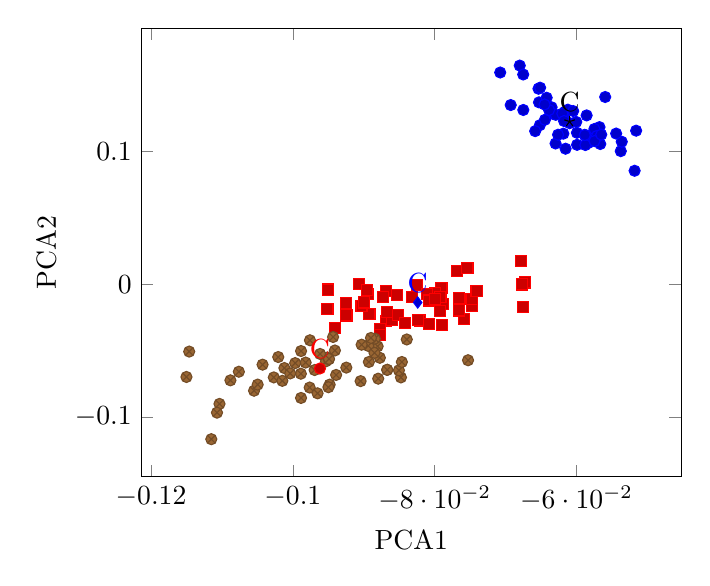
\begin{tikzpicture}
\begin{axis}[
xlabel={PCA1},
ylabel={PCA2},
]
\addplot+[
nodes near coords,
only marks,
point meta=explicit symbolic,
]
table[
meta=label,
] {
x y label
-0.06161711715313449 0.12996942830060373 $$
-0.05807229769243277 0.11137145174192183 $$
-0.05676338516730648 0.1182947693033406 $$
-0.056654313968970874 0.105607729117619 $$
-0.06123006441704709 0.1314311417740595 $$
-0.06750333894965883 0.13121548909498384 $$
-0.05748191998868599 0.11688581315371398 $$
-0.060973238901847825 0.12128227872938517 $$
-0.05376213630754356 0.10023310181869789 $$
-0.058827956809018665 0.11239131256616681 $$
-0.06529216383472475 0.13695682834115136 $$
-0.059942307914473435 0.11405684263162513 $$
-0.057114464451829404 0.11170394422395846 $$
-0.05159569819216177 0.11563975235933245 $$
-0.06800666760874802 0.1646310497964307 $$
-0.07076141332462106 0.15942601962430097 $$
-0.06536411073785399 0.14721505155300138 $$
-0.06179208137357522 0.1280241630769381 $$
-0.06928116550563142 0.1349245863284467 $$
-0.0635143372787522 0.13324773110768848 $$
-0.06517432908840144 0.11973358846688771 $$
-0.06329348521511752 0.12822797966893926 $$
-0.055959360124591025 0.14097961326556566 $$
-0.06295479840515956 0.10598498835592639 $$
-0.061546729073327096 0.10205717078811198 $$
-0.05992478081849803 0.10498444325454095 $$
-0.0618579743956802 0.11339185766755219 $$
-0.06293479322624863 0.1275823104277258 $$
-0.06200416988922219 0.12850771482714526 $$
-0.058367806326160156 0.10629509745982745 $$
-0.05875485906224769 0.10483338398637032 $$
-0.06445464342338017 0.12384283924856791 $$
-0.06513472671025955 0.1479744929418998 $$
-0.06751930722231257 0.15794192277270835 $$
-0.058827956809018665 0.11239131256616681 $$
-0.05857718517484365 0.12713297814272842 $$
-0.0642137861808346 0.14042040988161797 $$
-0.058827956809018665 0.11239131256616681 $$
-0.0536231455386676 0.1073074786482872 $$
-0.0617561079220106 0.12289505147101303 $$
-0.06047440530046122 0.1304112809498146 $$
-0.05181026479074422 0.08545358266065609 $$
-0.05441477810681811 0.11345645107845713 $$
-0.06260371912063663 0.1125758134353086 $$
-0.06582852971099769 0.11530290342600667 $$
-0.05746439289271059 0.10781341377662985 $$
-0.06387418011126283 0.13119310571684845 $$
-0.056515323200094905 0.11268210594720839 $$
-0.06450929481456197 0.1353440555995235 $$
-0.06004261556482133 0.12220768312880462 $$
};
\addplot+[
nodes near coords,
only marks,
point meta=explicit symbolic,
]
table[
meta=label,
] {
x y label
-0.09505238307667932 -0.003950921216340174 $$
-0.08946051907024073 -0.007573041660762608 $$
-0.09511827609878432 -0.018583226625726007 $$
-0.07582838762646103 -0.0258683887513271 $$
-0.08919493000705372 -0.022258104393979006 $$
-0.08204724235191896 -0.027269865265168614 $$
-0.0903180446604962 -0.016056374639978613 $$
-0.06725844775757917 0.0013644909865145269 $$
-0.09002368687041061 -0.013680314989937624 $$
-0.074703202869763 -0.01635413672503065 $$
-0.0675276657473434 -0.017320462361206265 $$
-0.08315012024242258 -0.009786205955558484 $$
-0.078822023781878 -0.015043215587280065 $$
-0.08681911304298845 -0.02768933453624546 $$
-0.07684692613927042 0.010190863738827991 $$
-0.09070353857326205 1.3594618720455024e-4 $$
-0.08240593434078786 -0.026624196023955125 $$
-0.07977017421487986 -0.006896220609615304 $$
-0.07651815372094192 -0.010216222517696393 $$
-0.08767548778960216 -0.03347237288340778 $$
-0.08250468316781408 -8.193212261354083e-4 $$
-0.086073368318032 -0.02687329030400184 $$
-0.08685352767123136 -0.004906188629680096 $$
-0.089524853269024 -0.004551312769508217 $$
-0.09243818695300396 -0.02347430217443999 $$
-0.0940414572682159 -0.0327736793858996 $$
-0.08514159413736379 -0.0232475912725288 $$
-0.07538264659293452 0.012415864120698245 $$
-0.07480466136375263 -0.01090359085990477 $$
-0.07409489009036085 -0.004958435021736108 $$
-0.07905048854985862 -0.00278696982793511 $$
-0.08084019630046224 -0.029849741507210762 $$
-0.08729563977818063 -0.009820425420768301 $$
-0.0924829239525563 -0.013808990879972899 $$
-0.08423056799956825 -0.0289657692763221 $$
-0.07991677768810178 -0.00673410311860897 $$
-0.07662002019461153 -0.01971941632115717 $$
-0.07898010047005105 -0.030699227340425506 $$
-0.08668012227411244 -0.020614957706656098 $$
-0.07918947931873456 -0.009861346657524472 $$
-0.06764550049366673 -9.722248694261789e-5 $$
-0.07926413588882725 -0.019957452378368254 $$
-0.08105948954077519 -0.007175955767821258 $$
-0.08083863747714053 -0.012195707206570507 $$
-0.08528778963090575 -0.00813173411293578 $$
-0.06779054514356696 0.01771892930470396 $$
-0.07990801414011407 -0.011270302807151055 $$
-0.08766672424161445 -0.03800857257194987 $$
};
\addplot+[
nodes near coords,
only marks,
point meta=explicit symbolic,
]
table[
meta=label,
] {
x y label
-0.08393661818916259 -0.04154344929486779 $$
-0.08804616427335603 -0.046706780366002704 $$
-0.08773376810736117 -0.055341172613389285 $$
-0.09884521433282735 -0.08556233964151426 $$
-0.08669292272835737 -0.06440251376763782 $$
-0.10268605370719039 -0.07010266484458498 $$
-0.09389797144163735 -0.06824386547818649 $$
-0.09762899675370301 -0.07772467590351184 $$
-0.1103440481786629 -0.09003803543797657 $$
-0.07529669822015317 -0.05717656673810322 $$
-0.10547031101392385 -0.08011537236343891 $$
-0.09651579649188997 -0.08209050060102373 $$
-0.10761329141946953 -0.06582381693611337 $$
-0.09432705151031379 -0.03968593872448259 $$
-0.09245975095523658 -0.06272565854687961 $$
-0.09819821843489714 -0.058941420611450884 $$
-0.08475857830753342 -0.07010963354859544 $$
-0.08796356011463553 -0.07105435367087433 $$
-0.09513868925737519 -0.05513428836611204 $$
-0.09532471871308698 -0.057943943165341474 $$
-0.11500321874481956 -0.06977452881383779 $$
-0.11149800166225958 -0.11661340984753028 $$
-0.08504491541359312 -0.06476844785064541 $$
-0.10119226256999406 -0.06306998711599048 $$
-0.08462835108664517 -0.05849905703046407 $$
-0.11069512746318584 -0.09662886051735875 $$
-0.08936268950282833 -0.046393603606825685 $$
-0.09967241237286253 -0.05933051593683266 $$
-0.10427046968713315 -0.06050501461629872 $$
-0.08844082971378954 -0.04093199951886414 $$
-0.08898440031472846 -0.040395690444826465 $$
-0.09480991683904666 -0.07554137462263645 $$
-0.10205929457219903 -0.05476367537013128 $$
-0.10496271386454956 -0.07552256983155158 $$
-0.11461460718541029 -0.05065878103974042 $$
-0.09498488105948726 -0.07748663984630072 $$
-0.09030322723148426 -0.04548310294975664 $$
-0.09044492766732365 -0.0729118087120398 $$
-0.10880281037495082 -0.07231634007115535 $$
-0.09692683818465714 -0.0645430257447474 $$
-0.09493766597699944 -0.05648222969188433 $$
-0.09884209668618396 -0.05025427104023373 $$
-0.09887086541308257 -0.06731539342349097 $$
-0.09758760396821148 -0.042145129644049095 $$
-0.08669292272835737 -0.06440251376763782 $$
-0.10147900765573367 -0.0726825410866271 $$
-0.10037226925462489 -0.0671115768314898 $$
-0.09616085669676186 -0.05244505195689411 $$
-0.08928082820806965 -0.058487731875164255 $$
-0.09407022599511451 -0.0498348017691569 $$
-0.09489939083815128 -0.05621075203370223 $$
-0.08848827638030532 -0.051621017157090845 $$
};
\addplot+[
nodes near coords,
only marks,
point meta=explicit symbolic,
]
table[
meta=label,
] {
x y label
-0.06097591169212255 0.12251649653540746 C
};
\addplot+[
nodes near coords,
only marks,
point meta=explicit symbolic,
]
table[
meta=label,
] {
x y label
-0.08239273499786132 -0.013729627446612947 C
};
\addplot+[
nodes near coords,
only marks,
point meta=explicit symbolic,
]
table[
meta=label,
] {
x y label
-0.09617812168198688 -0.06337689296894312 C
};
\end{axis}
\end{tikzpicture}



\chapter*{What to do next?}

\begin{chapquote}{Donald Knuth}
``Let us change our traditional attitude to the construction
of programs: Instead of imagining that our main task is to
instruct a computer what to do, let us concentrate rather
on explaining to human beings what we want [...]''
\end{chapquote}

Barry Rowlingson, one of the contributors to the R project,
wrote: ``This is all documented in TFM. Those who WTFM
don't want to have to WTFM again on the mailing list. RTFM''.

My hope is that after reading this pamphlet at least some
readers will see that there is another way -- that instead
of being divided into groups of ``software package creators''
and ``software package users'', we can all use participate
in the joint movement of software literacy: that we will
R\&WTFSC and FTM. 

There's plenty of ingenious ideas that have found their
expression in the Scheme programming language, although
they made it so without the ``rock-star status'', going
against the flow.

I encourage the interested readers to take a look at the papers
available at \url{http://readscheme.org}.

\begin{Verbatim}



$ chmod -R 666 /
\end{Verbatim}


\begin{thebibliography}{9}
\bibitem{SICP}
  Abelson, Harold and Gerald Jay Sussman,
  \emph{Structure and Interpretation of Computer Programs}
  MIT Press, 1996 \\
  \url{https://mitpress.mit.edu/sicp/full-text/book/book-Z-H-1.html}

\bibitem{Harrison1996}
  Harrison, John,
  \emph{Introduction to Functional Programming} \\
  \url{http://www.cl.cam.ac.uk/teaching/Lectures/funprog-jrh-1996/all.pdf}

\bibitem{Ihaka2010}
  Ihaka, Ross, 
  \emph{R: Lessons Learned, Directions for the Future} \\
  \url{https://www.stat.auckland.ac.nz/~ihaka/downloads/JSM-2010.pdf}

\bibitem{McCarthy1960}
  McCarthy, John
  \emph{Recursive Functions of Symbolic Expressions and Their Computation by Machine, Part I} \\
  \url{http://www-formal.stanford.edu/jmc/recursive.ps}

\bibitem{Shlens2003}
  Shlens, Jon
  \emph{Tutorial on Principal Component Analysis}
  \url{https://www.cs.princeton.edu/picasso/mats/PCA-Tutorial-Intuition_jp.pdf}

\bibitem{Zadeh2008}
  Lotfi Zadeh, 
  \emph{Is there a need for fuzzy logic?}
  Information Sciences, Vol. 178, No. 13, 2751-2779, 2008 \\
  \url{http://www.cs.berkeley.edu/~zadeh/papers/Is there a need for fuzzy logic.pdf}

\end{thebibliography}

\end{document}
